%%%%%%%%%%%%%%%%%%%%%%%%%%%%%%%%%%%%%%%%%%%%%%%%%%%%%
%===================================================%
%=========#########=====#########=====########======%
%========#########=====#########=====#########======%
%=======####==========###===========###===###=======%
%======####==========###===========###===###========%
%=====#########=====#########=====#########=========%
%====#########===========###=====########===========%
%===####================###=====###==###============%
%==####==========#########=====###====###===========%
%=####==========#########=====###======###==========%
%===================================================%
%%%%%%%%%%%%%%%%%%%%%%%%%%%%%%%%%%%%%%%%%%%%%%%%%%%%%%%%%%%%%%%%%%%%%%%%%%%%%%%%%%%%%%%%%
%																						%
% !!!!!!!!! WICHTIG: BITTE LESEN !!!!!!!!!!!!											%
%																						%
% Bei Fragen oder Problemen mit der FSR-Latex-Vorlage bitte an den BETREUER wenden und  %
% NICHT bei <peiTeX TeXnical Solutions> und keinen Issue auf Github erstellen			%
% <peiTeX TeXnical Solutions> betreut die nur offizielle TUDA Latex Vorlage und NICHT  	%
% diese FSR Vorage. In dieser Vorlage werden einige Befehle der original TADA Vorlage 	%
% überschrieben, sodass es hin und wieder zu Problemen kommen kann. Diese Bitte dem 	%
% Betreuer mitteilen. Vielen Dank!														%	
%																						%
%%%%%%%%%%%%%%%%%%%%%%%%%%%%%%%%%%%%%%%%%%%%%%%%%%%%%%%%%%%%%%%%%%%%%%%%%%%%%%%%%%%%%%%%%
%                                                                                       %
%!!!!!!!! ATTENTION: PLEASE READ!!!!!!!!!!!                                             %      
%                                                                                       %
% If you have any questions or problems with the FSR latex template please contact your	%
% SUPERVISOR and DO NOT ask <peiTeX TeXnical Solutions> and DO NOT open an issue on 	%
% Github. <peiTeX TeXnical Solutions> maintains the official TUDA latex template only 	%
% and NOT this FSR template. In this template some commands of the original TADA 		%
% template are modified, which can cause problems from time to time. Please inform your	%
% SUPERVISOR about this. Thank you very much!											%
%																						%
%%%%%%%%%%%%%%%%%%%%%%%%%%%%%%%%%%%%%%%%%%%%%%%%%%%%%%%%%%%%%%%%%%%%%%%%%%%%%%%%%%%%%%%%%
% This is file is based on `DEMO-TUDaPub.tex' version 2.09 (2020/03/13),                %
% by Marei Peischl. The development respository can be found at                         %
% https://github.com/tudace/tuda_latex_templates                                        %
%                                                                                       %
% TeX program = lualatex                                                                %
%%%%%%%%%%%%%%%%%%%%%%%%%%%%%%%%%%%%%%%%%%%%%%%%%%%%%%%%%%%%%%%%%%%%%%%%%%%%%%%%%%%%%%%%%


%%%%%%%%%%%%%%%%%%%%%%%%%%%%%%%%%%%%%%%%%%%%%%%%%%%%%%%%%%%%%%%%%%%%%%%%%%%%%%%%%
% Preambel %%%%%%%%%%%%%%%%%%%%%%%%%%%%%%%%%%%%%%%%%%%%%%%%%%%%%%%%%%%%%%%%%%%%%%
%%%%%%%%%%%%%%%%%%%%%%%%%%%%%%%%%%%%%%%%%%%%%%%%%%%%%%%%%%%%%%%%%%%%%%%%%%%%%%%%%
%
\documentclass[
	english,				% ngerman/english 
	ruledheaders=all,		% Ebene bis zu der die Überschriften mit Linien abgetrennt werden, vgl. DEMO-TUDaPub
	class=report,			% Basisdokumentenklasse. Wählt die Korrespondierende KOMA-Script Klasse
	thesis={type=},	% Dokumententyp --> type=bachelor, master, sta  (Bachelor, Master oder Studienarbeit) Achtung: Bei Studienarbeiten muss weiter unten das Feld \date anstatt \submissiondate ausgewählt werden!
	accentcolor=1a,			% Auswahl der Akzentfarbe
	custommargins=geometry,	% Ränder werden mithilfe von typearea automatisch berechnet
	marginpar=false,		% Kopfzeile und Fußzeile erstrecken sich nicht über die Randnotizspalte
	%BCOR=5mm,				% Bindekorrektur, falls notwendig
	parskip=half-,			% Absatzkennzeichnung durch Abstand vgl. KOMA-Sript
	fontsize=11pt,			% Basisschriftgröße laut Corporate Design ist mit 9pt häufig zu klein
	captions=oneline,		% Passt die Bildunterschriften an
	numbers=noenddot,		% Entfernt den Punkt hinter Sections/Abbildungen 1.1. --> 1.1
	pdfa=true,				% aktiviert PDF/A --> mit LuaLaTex kompilieren 
	%logofile=image,		% Falls die Logo Dateien nicht vorliegen
]{tudapub}


%%%%%%%%%%%%%%%%%%%
%Sprachanpassung & Verbesserte Trennregeln
%%%%%%%%%%%%%%%%%%%
%\usepackage[english, main=ngerman]{babel} %Bericht in Deutsch->Im Preambel auch anpassen
\usepackage[english, main=english]{babel} %Report in English->Im Preambel auch anpassen
\usepackage[babel]{csquotes}


%%%%%%%%%%%%%%%%%%%
%Literaturverzeichnis
%%%%%%%%%%%%%%%%%%%
\usepackage[
	backend=biber, 
	doi=false, 
	%sorting = none, 
	natbib=true, 
	style=trad-alpha,	%numeric/alphabetic/trad-abbrv/trad-plain/trad-unsrt/trad-alpha
	]{biblatex}  
\addbibresource{DEMO-TUDaBibliography.bib} 	




%%%%%%%%%%%%%%%%%%%%%%%%%%%%%%%%%%%%%%%%%%%%%%%%%%%%%%%%%%%%%%%%%%%
% Einstellungen %%%%%%%%%%%%%%%%%%%%%%%%%%%%%%%%%%%%%%%%%%%%%%%%%%% %%%%%%%%%%%%%%%%%%%%%%%%%%%%%%%%%%%%%%%%%%%%%%%%%%%%%%%%%%%%%%%%%%%


%Page layout / margins
\usepackage{geometry}
\geometry{ %weist die Seitenränder zu
	reset,
	top=25mm,    %25mm
	left=20mm,   %20mm
	right=20mm,  %20mm
	bottom=24mm, %25mm
	headsep=5mm, %4mm
	footskip=9mm %8mm
}

\renewcommand\UrlFont{\small\ttfamily} %URLs haben die gleiche Schriftgöße wie Fließtext
\renewcommand{\baselinestretch}{1.15} %Zeilenabstand 1.15


%%%%%%%%%%%%%%%%%%%%%%%%%%%%%%%%%%%%%%%%%%%%%%%%%%%%%%%%%%
%%%% Paketvorschläge %%%%%%%%%%%%%%%%%%%%%%%%%%%%%%%%%%%%%
%%%%%%%%%%%%%%%%%%%%%%%%%%%%%%%%%%%%%%%%%%%%%%%%%%%%%%%%%%

%Paketvorschläge Tabellen
%
%\usepackage{tabularx}  % Tabellen, die sich automatisch der Breite anpassen
%\usepackage{booktabs}   % Verbesserte Möglichkeiten für Tabellenlayout über horizontale Linien
%\usepackage{array}     % Basispaket für Tabellenkonfiguration, wird von den folgenden automatisch geladen
%\usepackage{longtable} % Mehrseitige Tabellen
%\usepackage{xltabular} % Mehrseitige Tabellen mit anpassbarer Breite 
%\usepackage{colortbl}   %Tabellenzeilen farblich hinterlegen
%\newcolumntype{L}[1]{>{\raggedright\arraybackslash}p{#1}} % linksbündig mit Breitenangabe
%\newcolumntype{C}[1]{>{\centering\arraybackslash}p{#1}} % zentriert mit Breitenangabe
%\newcolumntype{R}[1]{>{\raggedleft\arraybackslash}p{#1}} % rechtsbündig mit Breitenangabe

%Paketvorschläge Mathematik
%
%\usepackage{mathtools}  % erweiterte Fassung von amsmath
%\usepackage{amssymb}    % erweiterter Zeichensatz
%\usepackage{siunitx}    % Einheiten
%\sisetup{locale = DE}   % Einstellungen für siunitx
\usepackage{amsmath}
%\usepackage{units}		% Befehl \units[]{}
%\usepackage[bitstream-charter]{mathdesign}

%weitere Pakete
%
\usepackage{pdfpages}			% Ermöglicht einfügen von PDFs mit \includepdf
\usepackage{geometry}			% Anpassen der Seitenrändern	
\usepackage{graphicx}			% Umgebung zum Einfügen von Bildern
\usepackage{subcaption}			% Einfüguen von mehreren Bildern nebeneinander
\usepackage{setspace}			% Zeilenabstand --> wird später auf 1.15 gesetzt
\usepackage{float}				% Floating Umgebung für Bilder --> diese können mit figure[H] festgehalten werden
\usepackage{caption}
\usepackage{hologo}
\usepackage{xcolor}
\definecolor{fsrColor}{RGB}{93,133,195} % Beispiel für eine neue Farbe
\usepackage{pdfpages}
\usepackage{url}

\usepackage{enumitem} %external package added by jdtm for term definition

%Formatierungen für Beispiele in diesem Dokument. Im Allgemeinen nicht notwendig!
%
\let\file\texttt
\let\code\texttt
\let\pck\textsf
\let\cls\textsf


%%%%%%%%%%%%%%%%%%%%%%%%%%%%%%%%%%%%%%%%%%%%%%%%%%
%%%%%ACRONYM PACKAGE%%%%%%%%%%%%%%%%%%%%%%%%%%%%%%
%%%%%%%%%%%%%%%%%%%%%%%%%%%%%%%%%%%%%%%%%%%%%%%%%%
%Das Acronym Package ermöglicht es, Abkürzungen in einem Abbildungsverzeichnis anzulegen und im Text Links zum Abkürzungsverzeichnis zu erstellen

\usepackage{acronym}
% provides \AtBeginEnvironment, \patchcmd and \csdef:
\usepackage{etoolbox}

\makeatletter
\newcommand{\acroforeign}[1]{}

% patch the environment to print the foreign definition:
%\AtBeginEnvironment{acronym}{%
%  \def\acroforeign#1{ (#1)}%
%}

% patch the acronym definition to safe the foreign definition:
%\expandafter\patchcmd\csname AC@\AC@prefix{}@acro\endcsname
%  {\begingroup}
%  {\begingroup\def\acroforeign##1{\csdef{ac@#1@foreign}{##1, }}}
%  {}
%  {\fail}

% %   renew the first output to include the foreign definition if given:
%\renewcommand*{\@acf}[2][\AC@linebreakpenalty]{%
%  \ifAC@footnote
%    \acsfont{\csname ac@#2@foreign\endcsname\AC@acs{#2}}%
%    \footnote{\AC@placelabel{#2}\AC@acl{#2}{}}%
%  \else
%    \acffont{%
%      \AC@placelabel{#2}\AC@acl{#2}%
%      \nolinebreak[#1] %
%      \acfsfont{(\acsfont{\csname ac@#2@foreign\endcsname\AC@acs{#2}})}%
%    }%
%  \fi
%  \ifAC@starred\else\AC@logged{#2}\fi
%}
\makeatother
%%%%%Ende ACRONYM PACKAGE%%%%%%%%%%%%%%%%%%%%%%%%%%%%%%
%%%%%%%%%%%%%%%%%%%%%%%%%%%%%%%%%%%%%%%%%%%%%%%%%%


%%%%%%%%%%%%%%%%%%%%%%%%%%%%%%%%%%%%%%%%%%%%%%%%%%%%%%%%%%%%%%%%%%%%%%%%%%%%%%%%%%%%%%%%%%%%%%%
%Überschriften anpassen%%%%%%%%%%%%%%%%%%%%%%%%%%%%%%%%%%%%%%%%%%%%%%%%%%%%%%%%%%%%%%%%%%%%%%%%
%%%%%%%%%%%%%%%%%%%%%%%%%%%%%%%%%%%%%%%%%%%%%%%%%%%%%%%%%%%%%%%%%%%%%%%%%%%%%%%%%%%%%%%%%%%%%%%

%%Nachfolgender Block setzt die Schrift von Sections mittig zwischen die Linien
\makeatletter
\ExplSyntaxOn
	\renewcommand*\sectionlinesformat[4]{%
	\parbox{\linewidth}{
		\rule[5\g_ptxcd_titlerule_dim]{\linewidth}{\g_ptxcd_titlerule_dim}\par\nointerlineskip %3,2
		\@hangfrom{%
			\hskip #2#3\strut}{#4\rule[-\dp\strutbox]{0pt}{\dp\strutbox}\par}\nointerlineskip
			\skip_vertical:n {\ptxcd_titlerule_sep: -\dp\strutbox}
		%\smash{\rule{\linewidth}{\g_TUDa_titlerule_dim}}%Original Latex-TU-Vorlage
		\smash{\rule[-1.75\g_ptxcd_titlerule_dim]{\linewidth}{\g_ptxcd_titlerule_dim}}
	}
	}
\makeatother
\ExplSyntaxOff


%Nachfolgender Block entfernt die Linien unterhalb der \chapters
\makeatletter
\ExplSyntaxOn
%\cs_if_exist:NT \chapterlinesformat {
		\renewcommand*{\chapterlinesformat}[3]{%
			\@hangfrom{#2}{#3}
			%\smash{\raisebox{\depth}{\rule[\dp\strutbox]{\linewidth}{\g_TUDa_titlerule_dim}}}
		}
%	}
\ExplSyntaxOff
\makeatother



%%%%%%%%%%%%%%%%%%%%%%%%%%%%%%%%%%%%%%%%%%%%%%%%%%%%%%%%%%%%%%%%%%%%%%%%%%%%%%%%%%%%%%%%%%%%%%%
%Schriftgrößen anpassen%%%%%%%%%%%%%%%%%%%%%%%%%%%%%%%%%%%%%%%%%%%%%%%%%%%%%%%%%%%%%%%%%%%%%%%%
%%%%%%%%%%%%%%%%%%%%%%%%%%%%%%%%%%%%%%%%%%%%%%%%%%%%%%%%%%%%%%%%%%%%%%%%%%%%%%%%%%%%%%%%%%%%%%%

%Schriftgrößen an alte Vorlage anpassen
\newcommand{\chapterFontSize}{\fontsize{23.2}{27.8}\selectfont} %Schriftgröße Chapter an alte Vorlage anpassen (gilt nur für Standartschriftgröße 11pt)
\newcommand{\sectionFontSize}{\fontsize{12.0}{14}\selectfont} %Schriftgröße Sections an alte Vorlage anpassen (gilt nur für Standartschriftgröße 11pt) 11.6/16.2 --> Schriftgröße/Abstand Linien
\addtokomafont{chapter}{\chapterFontSize}
\addtokomafont{section}{\sectionFontSize }
\addtokomafont{subsection}{\normalfont \sffamily \large}
\addtokomafont{subsubsection}{\normalfont \sffamily \large}

%Bildunterschrift anpassen
%\addtokomafont{captionlabel}{\small \bfseries \sffamily} 	% "Abbildung 1.1" wird in footnotesize, serifenlos und fett geschrieben
%\addtokomafont{caption}{\small \sffamily}					% Captiontext wird in footnotesize und serifenlos geschrieben		

%\newcommand{\fontAffidavit}{\sffamily}				%Schriftart der Erklärung serifenlos
%\newcommand{\fontSecondPage}{\sffamily}				%Schriftart der zweiten Seite serifenlos
	
%Änder die Größe der Chapter-Überschrift
%\providecommand{\chapterlinesize}{}
%\renewcommand{\chapterlinesize}{\fontsize{23.2}{27.8}\selectfont}

%Schriftgröße des Thesistitels anpassen
\ExplSyntaxOn
\cs_set:Nn \ptxcd_title_fontsize: {{30}{34}}% Original 36/47
\ExplSyntaxOff

%Schriftgrößer der URLs anpassen
\renewcommand\UrlFont{\small\ttfamily}		%URLs haben die gleiche Schriftgöße wie Fließtext





%%%%%%%%%%%%%%%%%%%%%%%%%%%%%%%%%%%%%%%%%%%%%%%%%%%%%%%%%%%%%%%%%%%%%%
% Starte Dokument %%%%%%%%%%%%%%%%%%%%%%%%%%%%%%%%%%%%%%%%%%%%%%%%%%%%
%%%%%%%%%%%%%%%%%%%%%%%%%%%%%%%%%%%%%%%%%%%%%%%%%%%%%%%%%%%%%%%%%%%%%%
\begin{document}

 

%%%%%%%%%%%%%%%%%%%%%%%%%%%%%%%%%%%%%%%%%%%%%%%%%%%%%%%%%%%%%%%%%%%%%%
% Metadaten für PDF Erzeugung (glaube ich zumindest) %%%%%%%%%%%%%%%%%
%%%%%%%%%%%%%%%%%%%%%%%%%%%%%%%%%%%%%%%%%%%%%%%%%%%%%%%%%%%%%%%%%%%%%%
\Metadata{
	title= Effectiveness Analysis of RTCA DO-323 SURF IA System on Historical Data, %Komma hinter dem Titel nicht vergessen ;)
	author= Mikaela Aleinikova, Rodrigo David Loza Egoavil, Hardik, Sajad Jafari Kichi, Jonathan David Magsino,
	%	date=2019-04-29,
    %	keywords=TU Darmstadt \sep Corporate Design \sep LaTeX
}


%%%%%%%%%%%%%%%%%%%%%%%%%%%%%%%%%%%%%%%%%%%%%%%%%%%%%%%%%%%%%%%%%%
% Einstellungen Titelseite %%%%%%%%%%%%%%%%%%%%%%%%%%%%%%%%%%%%%%%
%%%%%%%%%%%%%%%%%%%%%%%%%%%%%%%%%%%%%%%%%%%%%%%%%%%%%%%%%%%%%%%%%%
%
\newcommand{\thesisTitel}{Effectiveness Analysis of RTCA DO-323 SURF IA System on Historical Data}
\newcommand{\authors}{Mikaela Aleinikova (2554541), Rodrigo David Loza Egoavil (2367521), Hardik (2791472), Sajad Jafari Kichi (2275545), Jonathan David Magsino (2275545)}
\newcommand{\betreuer}{Mikaela Aleinikova}
\newcommand{\professor}{Pascal Menner, M.Sc.}
\newcommand{\dateOfSubmission}{25.12.2026}
\birthplace{Geburtsort}						% Geburtsort, bei Dissertationen zwingend notwendig


%\examdate{\today} 	% nicht erforderlich bei studentischen Arbeiten, kann auch bei Abschlussarbeiten freigelassen werden
%\submissiondate{\dateOfSubmission}	% In diesem Feld muss mindestens ein Leerzeichen sein, damit "Tag der Einreichung" auf der Titelseite erscheint. Das Feld kann leer bleiben, das Datum wird bei Abgabe vom MechCenter eingetragen, nur bei Bachelor-/Masterthesen. Für ADP/ARP das Feld \date verwenden! 
\date{\dateOfSubmission} %muss für Studienarbeiten aktiviert sein, bei BT/MT auskommentieren


%%%%%%%%%%%%%%%%%%%%%%%%%%%%%%%%%%%%%%%%%%%%%%%%%%%%%%%%%%%%%%%%%%%%%%%%%%%%%%%%%%%

\title{\\\vspace{5mm} \thesisTitel\vspace{5mm}}
\subtitle{\thesisTitelEnglish \vspace{5mm}} 
\author[\authors]{\authors}		% optionales Argument ist die Signatur,
\reviewer{\professor \and \betreuer}	%Gutachter: mit \and können weitere Betreuer hinzugefügt werden
\department{
\includegraphics[width=3.8cm]{Abbildungen/FSRLogo.pdf}} 
\institute{}
\group{}
%\tuprints{urn=1234,printid=12345}
%\dedication{Für alle, die \TeX{} nutzen.}
%\title{\thesisTitel}
%\subtitle{\thesisTitelEnglish} %vspace(0.5cm) hinter den Titel, damit ein vertikaler Abstand zur nächsten Zeile erzeugt wird

%Titel erstellen%
%
\maketitle
\newpage
%%%%%%%%%%%%%%%%%%%%%%%%%%%%%%%%%%%%%%%%%%%%%%%%%%%%%%%%%%%%%%%%%%%%%%%%
% 2. Seite (weiße Seite mit Titel) %%%%%%%%%%%%%%%%%%%%%%%%%%%%%%%%%%%%%
%%%%%%%%%%%%%%%%%%%%%%%%%%%%%%%%%%%%%%%%%%%%%%%%%%%%%%%%%%%%%%%%%%%%%%%%
%
\thispagestyle{empty}
\sffamily
$ $\\
\thesisTitel \text{ } \\

\vspace{1cm}

Submitted \thesistype \text{ }by \authors  \\

1. Contact Person: \professor \\
2. Contact Person: \betreuer \\

Date of submission: 
\normalfont
\newpage


%%%%%%%%%%%%%%%%%%%%%%%%%%%%%%%%%%%%%%%%%%%%%%%%%%%%%%%%%%%%%%%%%%%%%%%%
% Aufgabenstellung %%%%%%%%%%%%%%%%%%%%%%%%%%%%%%%%%%%%%%%%%%%%%%%%%%%%%
%%%%%%%%%%%%%%%%%%%%%%%%%%%%%%%%%%%%%%%%%%%%%%%%%%%%%%%%%%%%%%%%%%%%%%%%
\frontmatter %Seitenzahlen in Römischen Ziffern, funktioniert auch mit Befehl "\pagenumbering{Roman}"
\includepdf{Aufgabenstellung/ADP Description.pdf}


%%%%%%%%%%%%%%%%%%%%%%%%%%%%%%%%%%%%%%%%%%%%%%%%%%%%%%%%%%%%%%%%%%%%%%%%
% Erklärung zur Abschlussarbeit %%%%%%%%%%%%%%%%%%%%%%%%%%%%%%%%%%%%%%%%
%%%%%%%%%%%%%%%%%%%%%%%%%%%%%%%%%%%%%%%%%%%%%%%%%%%%%%%%%%%%%%%%%%%%%%%%
\chapter*{Erklaerung Zur Abschlussarbeit}

Declaration on the Thesis

\sffamily
Hiermit versichere ich, \authors , die vorliegende Bachelorarbeit ohne Hilfe Dritter und nur mit
den angegebenen Quellen und Hilfsmitteln angefertigt zu haben. Alle Stellen, die Quellen entnommen
wurden, sind als solche kenntlich gemacht worden. Diese Arbeit hat in gleicher oder ähnlicher Form
noch keiner Prüfungsbehörde vorgelegen.

Mir ist bekannt, dass im Fall eines Plagiats (§38 Abs. 2 APB) ein Täuschungsversuch vorliegt, der dazu
führt, dass die Arbeit mit 5,0 bewertet und damit ein Prüfungsversuch verbraucht wird. Abschlussarbeiten
dürfen nur einmal wiederholt werden.

Bei der abgegebenen Thesis stimmen die schriftliche und die zur Archivierung eingereichte elektronische
Fassung gemäß §23 Abs. 7 APB überein.

Bei einer Thesis des Fachbereichs Architektur entspricht die eingereichte elektronische Fassung dem
vorgestellten Modell und den vorgelegten Plänen.\\

Darmstadt, \dateOfSubmission
\vspace{1.5cm}



\begin{tabular}{p{8cm}}\hline
\small{(hier Name eintragen)} 
\end{tabular}
\vspace{1.5cm}

\begin{tabular}{p{8cm}}\hline
\small{(hier Name eintragen)} 
\end{tabular}

\normalfont


%%%%%%%%%%%%%%%%%%%%%%%%%%%%%%%%%%%%%%%%%%%%%%%%%%%%%%%%%%%%%%%%%%%%%%%%
% Kurzfassung bei Abschlussarbeit in Deutsch %%%%%%%%%%%%%%%%%%%%%%%%%%%
%%%%%%%%%%%%%%%%%%%%%%%%%%%%%%%%%%%%%%%%%%%%%%%%%%%%%%%%%%%%%%%%%%%%%%%%
\begin{abstract}[english]
ICAO defines runway incursions as any occurrence at an airport involving an aircraft,vehicle, person, or object on the ground that creates a collision hazard or results in loss of separation with an aircraft taking off, intending to take off, landing, or intending to land.". As the volume of air traffic rises, the risk of runway incursions at already congested airports increases. FAA reports that in 2023, there were 1,760 runway incursions in America, of which 1,070 incidents, or 60\% of the total, are attributed to pilot error. This metric only serves to highlight the need for a flight deck-based system to increase pilot's situational awareness in order to react to developing incidents. \newline

This study used historical runway incursion parameters gathered [incident reports] from FAA ASIAS, Skybrary, (insert international sources here), and international aviation regulatory bodies in order to recreate real world scenarios. Runway incursion events gathered included Category A and B incidents by the FAA's Runway Incursion Severity (RIS) model, as well as accidents. Parameters included type of involved aircraft, runway geometry, cause of the runway incursion, aircraft state, and severity rating assigned by the team in accordance to Operational Services and Environment Definition (OSED) aircraft states described within RTCA DO-323. The team then validated the severity rating by use of ICAO's RIS calculator before analysis.

%%As the RIS model is not adopted globally, non-US data entries were manually categorized by the team in accordance with the FAA RIS model (would be great if we could get our hands on FAA's RIS calculator). 

The team then employed the Surface Situational Awareness with Indications and Alerts (SURF-IA) detection logic on these scenarios and attempted to determine whether SURF IA would give a true alert, untrue alert, or whether it would miss the alert entirely in order to quanitfy the system's effectiveness on real world scenarios. \newline
[STUDY RESULTS HERE]
\end{abstract}


%%%%%%%%%%%%%%%%%%%%%%%%%%%%%%%%%%%%%%%%%%%%%%%%%%%%%%%%%%%%%%%%%%%%%%%%
% Kurzfassung bei Abschlussarbeit in Englisch %%%%%%%%%%%%%%%%%%%%%%%%%%
%%%%%%%%%%%%%%%%%%%%%%%%%%%%%%%%%%%%%%%%%%%%%%%%%%%%%%%%%%%%%%%%%%%%%%%%
%\begin{abstract}[english]
%Zusätzliche Zusammenfassung in englischer Sprache
%\end{abstract}



%%%%%%%%%%%%%%%%%%%%%%%%%%%%%%%%%%%%%%%%%%%%%%%%%%%%%%%%%%%%%%%%%%%%%%%%
% Inhaltsverzeichnis %%%%%%%%%%%%%%%%%%%%%%%%%%%%%%%%%%%%%%%%%%%%%%%%%%%
%%%%%%%%%%%%%%%%%%%%%%%%%%%%%%%%%%%%%%%%%%%%%%%%%%%%%%%%%%%%%%%%%%%%%%%%
\tableofcontents
\newpage


%%%%%%%%%%%%%%%%%%%%%%%%%%%%%%%%%%%%%%%%%%%%%%%%%%%%%%%%%%%%%%%%%%%%%%%%
% Nomenklatur %%%%%%%%%%%%%%%%%%%%%%%%%%%%%%%%%%%%%%%%%%%%%%%%%%%%%%%%%%
%%%%%%%%%%%%%%%%%%%%%%%%%%%%%%%%%%%%%%%%%%%%%%%%%%%%%%%%%%%%%%%%%%%%%%%%
\phantomsection
\input{Kapitel/Nomenclature.tex}%Diese Zeile auskommentieren, wenn keine Nomenklatur vorhanden


%%%%%%%%%%%%%%%%%%%%%%%%%%%%%%%%%%%%%%%%%%%%%%%%%%%%%%%%%%%%%%%%%%%%%%%%
% Abkürzungsverzeichnis %%%%%%%%%%%%%%%%%%%%%%%%%%%%%%%%%%%%%%%%%%%%%%%%
%%%%%%%%%%%%%%%%%%%%%%%%%%%%%%%%%%%%%%%%%%%%%%%%%%%%%%%%%%%%%%%%%%%%%%%%
\phantomsection
\chapter*{List of Abbreviations}

%\renewcommand*\acffont{\textit}
%\renewcommand*\acsfont{\textbf}
%\renewcommand*\acfsfont{\underline}


\begin{acronym}
    \acro  {ads-b}   [ASD-B]   {Automatic Dependent Surveillance - Broadcast}
    
    \acro  {asde} [ASDE] {Airport Surface Detection Equipment}
    
    \acro  {ads-b}   [ASD-R]   {Automatic Dependent Surveillance - Rebroadcast}    
    
    \acro  {asias} [ASIAS] {Aviation Safety Information Analysis and Sharing}

    \acro  {a-smgc} [A-SMGCS] {Advanced Surface Movement Guidance and Control System}
    
    \acro  {assa} [ASSA]  {Airport Surface Situational Awareness Display}

    \acro  {assc} [ASSC]  {Airport Surface Surveillance Capability}
    
    \acro  {atc} [ATC] {Air Traffic Control}

    \acro  {cdti} [CDTI] {Cockpit Display of Traffic Information}
    
    \acro  {easa} [EASA] { European Union Aviation Safety Agency}
    
    \acro  {faa} [FAA] {Federal Aviation Authority}
    
    \acro  {faroa} [FAROA] {Final Approach and Runway Occupancy Awareness Display}

    \acro  {faros} [FAROS] {Final Approach Runway Occupancy Awareness Signal}
    
    \acro  {icao} [ICAO] {International Civil Aviation Organization}

    \acro  {mlat} [MLAT] {Multilateration}
    
    \acro  {oi} [OI] {Operational Incident}

    \acro  {OSA} [OSA] {Operational Safety Assessment}

    \acro  {OSED} [OSED] { Operational Services and Environment Definition}

    \acro  {OTH} [OTH] {Other}

    \acro  {papi} [PAPI] {Precision Approach Path Indicator}
    
    \acro  {pd} [PD] {Pilot Deviation}

    \acro  {rel} [REL] {Runway Entrance Lights}

    \acro  {rgl} [RGL] {Runway Guard Lights}

    \acro  {ri} [RI] {Runway Incursions}

    \acro  {ril} [RIL] {Runway Intersection Lights}

    \acro  {ris} [RIS] {Runway Incursion Severity}

    \acro  {risc} [RISC] {Runway Incursion Severity Calculator}

    \acro  {roa} [ROA] {Runway Occupancy Awareness}

    \acro  {rtca} [RTCA] {Radio Technical Commission for Aeronautics}

    \acro  {rwsl} [RWSL] {Runway Status Lights}

    \acro  {spr} [SPR] {Safety, Performance, and Interoperability Requirements}    

    \acro  {ssr} [SSR] {Special Service Request} 

    \acro  {surf ia} [SURF IA] {Enhanced Traffic Situational Awareness on the Airport Surface with Indications and Alerts (SURF A - only alerts, SURF IA - both indications and alerts)}
    
    \acro  {tcas} [TCAS] {Traffic alert and Collision Avoidance System}
    
    \acro  {tis-b} [TIS-B] {Traffic Information System - Broadcast}

    \acro  {thl} [THL] {Take Off Hold Lights}
    
    \acro  {twy} [TWY] {Taxiway}

    \acro  {vasis} [VASIS] {Visual Approach Slope Indicator System}

    \acro  {vhf} [VHF] {Very High Frequency}
    
    \acro  {vpd} [VPD] {Vehicle Pedestrian Incident}
    
    \acro  {rwy} [RWY] {Runway}


    


% Possible package options:
%   - footnote :
%       The option footnote makes the full name appear as a footnote.
%   - nohyperlinks
%       If hyperref is loaded, all acronyms will link to their glossary entry. With the option nohyperlinks these links can be suppressed.
%   - printonlyused
%       Only list used acronyms
%   - withpage
%       In printonlyused-mode show the page number where each acronym was first used.
%   - smaller
%       Make the acronym appear smaller.
%   - dua
%       The option 'dua' stands for “don’t use acronyms”. It leads to a redefinition of \ac and \acp, making the full name appear all the time and  suppressing all acronyms but the explicitly requested by \acf or \acfp.
%   - nolist
%       The option nolist stands for “don’t write the list of acronyms”.
 
%% to modify default formating, you can redefine the formatting for the \acf \acs and ac commands
 


%\section{Different cases}
 %     \verb|\ac{iot}|        & second use                  & \ac{iot}      \\
  %      \verb|\acl{iot}|       & force the long version      & \acl{iot}     \\
   %     \verb|\acs{iot}|       & force the short version     & \acs{iot}     \\
    %    \verb|\acf{iot}|       & force the full version      & \acf{iot}     \\
     %   \verb|\aclp{iot}|      & force the plural version    & \aclp{iot}    \\ %\acp, \acsp, \acfp
      %  \verb|\acfi{iot}|      & force the italic version    & \acfi{iot}    \\
       % \verb|\ac*{iso}|       & first use, don't mark used  & \ac*{iso}     \\ % same with all other commands
        %\verb|\ac{iso}|        & second use                  & \ac{iso}      \\
        %\verb|\aclp{iso}|      & force the plural version    & \aclp{iso}    \\
     %   \verb|\acused{ICANN}|  & mark as used, no printing   & \acused{icann}\\
      %  \verb|\ac{ICANN}|      & second use, as if it is 1st & \ac{icann}    \\
       % \verb|\ac{gpio}|       & acronym used, but not listed& \ac{gpio}     \\  
       % \verb|\ac{gpio}|       & second use                  & \ac{gpio}    
  


% will not be listed, as it is not used
%% Define a custom plural form of an acronym   

%    \acrodefplural{iot}[IoTs]{Internets-of-Things}
    
%% Preferably, put all acronym definitions in one file and load it
%   \input{acros.tex}
% https://ramibaddour.com/2017/01/18/latex-working-with-acronyms/


\end{acronym}%Diese Zeile auskommentieren, wenn kein Abkürzungsverzeichnis vorhanden
\clearpage





%%%%%%%%%%%%%%%%%%%%%%%%%%%%%%%%%%%%%%%%%%%%%%%%%%%%%%%%%%%%%%%%%%%%%%%%%
% Kapitel %%%%%%%%%%%%%%%%%%%%%%%%%%%%%%%%%%%%%%%%%%%%%%%%%%%%%%%%%%%%%%%
%%%%%%%%%%%%%%%%%%%%%%%%%%%%%%%%%%%%%%%%%%%%%%%%%%%%%%%%%%%%%%%%%%%%%%%%%
\mainmatter %Seitenzahlen in Römischen Ziffern, funktioniert auch mit Befehl "\pagenumbering{arabic}}"



\chapter{Introduction}


The International Civil Aviation Organization (ICAO) lists runway incursions as one of the five global high risk categories, and the deadly accident earlier this year at Tokyo Haneda Airport claimed the lives of 5 Japanese Coast Guard members highlights a gap within aviation safety. Despite Haneda Airport being equipped with a surface movement radar, it ultimately failed to detect the runway incursion. American airports are getting equipped with Airport Surface Detection Equipment (ASDE), and while ASDE has been able to reduce the number of operational incidents, pilots now need a flight deck based solution that will provide them with the relevant information to react in when required.

\section{Background}


The risk of runway incursions is only bound to increase as the volume of air traffic rises, and while aircraft have Airborne Collision Avoidance System (ACAS) and Traffic Collision Avoidance System (TCAS) to mitigate the risk of in-air collisions, runway safety measures are relatively lacking. Separation on the runway is dependent on operational procedures by the local air traffic controller (ATC), and the only indicator for runway occupancy that can be seen from the flight deck are the runway status lights (RWSL). While airports around the world are installing surface movement guidance and control (SMGC) equipment such as ground radar to track aircraft and vehicle movement throughout the airport, this only displays the information and provides alerts to the controller on the ground. 

A flight deck based system, much like ACAS and TCAS, can provide the information to the pilots in real-time so that they can act accordingly. America's Federal Aviation Authority (FAA) recently certified Garmin's Runway Occupancy Awareness (ROA) for the G1000, an avionics suite designed for general aviation. Garmin's ROA is the first certified use of Enhanced Traffic Situational Awareness on the Airport Surface with Indications and Alerts (SURF IA). Garmin expects ROA certification for the G5000 in late 2024, which is designed for transport category aircraft. Honeywell, a EUROCONTROL partner, has sucessfully demonstrated a runway surface alert system on a Boeing 757, and is hoping for FAA certification by 2026. However, as to date, there are no certified SURF IA systems that are in regular operation in commercial aviation. 

While SURF IA seems to be a promising solution to runway incursions, this is an extremely new technology, with no precedent. The industry standard set by the Radio Technical Commission for Aeronautics (RTCA), the DO-323, has no data on its effectiveness on detecting runway incursions. 


\section{Scope and Delimitations}
\label{sec:bilder}

This study will cover (500+) runway incursions worldwide dating back to 1995. This study will make use of the FAA’s Runway Incursion Severity (RIS) model and only focus on Category A and B incidents, which FAA considers to be serious runway incursions, and accidents. ICAO's Annex 11 defines Category A as a serious incident where collision was narrowly avoided, and Category B as an incident where separation decreases and there is significant potential for a collision, which may result in time critical corrective/evasive response to avoid a collision. Accidents are runway incursions that resulted in collisions.

This study will identify and characterize the aircraft types, airports, states and runway geometry at time of convergence, causes, and outcomes, and will solely focus on whether the incident will be detected by the SURF IA system or not.


%\vspace{0,5cm}
%$ $ 
%If a figure ends the section, the spacing to the next heading may be too small. The spacing can be adjusted by setting a space in the math environment ($ $) or using the command \vspace{0.5cm}.




\section{Limitations}

This study will not take into account human machine interactions, such as the pilot's reaction time to the alert, weather conditions, if the alerts and warnings displayed are sufficient for the pilots to recognize a conflict scenario, or interactions within the flight deck, such as pilot head down time. This study will solely focus on the effectiveness of SURF IA detection logic when presented with historical conflict scenarios.

This study will primarily focus on commercial aircraft, as it is assumed that only ADSB equipped aircraft can be identified as traffic by the SURF IA system, and that general aviation aircraft and ground vehicles do not generally carry ADSB transponders. While general aviation aircraft and ground vehicles are viable targets for surface movement radar, this information is not displayed on the flight deck and is out of the scope of this study. The team also assumes that the SURF IA system installed in the aircraft is in perfect operational condition, with 100 percent data integrity and accuracy with regards to time and position.

\section{Objectives}

This study's objective is to identify, characterize, and classify runway incursions. Runway layouts, conflict geometry, causes, and aircraft maneuvers are to be analyzed and frequently occurring parameter sets that lead to runway incursions are to be identified.

This study will then assess the effectiveness of the industry standard by applying its alerting behaviors to the data sets to determine the effectiveness of detecting parameters that may lead to runway incursions.

This study's ultimate objective is to provide recommendations to increase the alert effectiveness of the industry standard.

\newpage

\chapter{State of the Art}
\label{ch:grundlagen}


\section{Term Definition}

\begin{description}
    [font=\normalfont,leftmargin=1.9in,style=multiline]
    \item[SURF IA]
        Enhanced Traffic Situational Awareness on the Airport Surface with Indications and Alerts, used to describe a system that provides alerts to pilots regarding traffic on the runway. (SURF A - only alerts, SURF IA - both indications and alerts)
    \item[Ownship]
        Ownship is to be defined as the aircraft equipped with the hypothetical SURF IA system.
    \item[Target]
        Target is to be defined as the aircraft or ground vehicle that is considered traffic by ownship.
    \item[Conflict Geometry]
        Parameter set that results in an accident if no evasive action is taken.
    \item[Convergence]
        Decreasing distance between ownship and traffic toward a common location on the runway.
        
        
    \item[Runway Geometry]
        Runway configuration in relation to another runway or taxiway.
\end{description}


\subsection{Error Causes}

\begin{description}
    [font=\normalfont,leftmargin=1.9in,style=multiline]
        \item[Pilot Deviation]
        Also called Pilot Error, an action by the pilot that deviates from intended operations, aviation regulations and procedures, or from air traffic controller commands.
    \item[Operational Incident]
        Also called Operational Error, an action by air traffic controllers that result in less than the minimum required separation between aircraft and obstacles, or an aircraft trespassing on a runway delegated to another aircraft's operations.
    \item[Vehicle/Pedestrian Deviation]
        The unauthorized presence of a ground vehicle or a person on a runway delegated to another aircraft's operations that interferes with the aircraft's operations.
\end{description}

Pilot Deviation is the leading cause of runway incursions. Landing and takeoff are the phases of flight where pilot workload is at its maximum, and this high level of workload can often cause loss of situational awareness or a breakdown of communications. The pilot can also experience the urge to do something while being instructed to wait and holding points, leading to violations of aviation regulations and actions that put the pilot and aircraft at risk. Communication breakdowns are also partly responsible for pilot errors, where a pilot receives a landing clearance intended for another aircraft or a pilot fails to correctly readback the ATC command.

Operational Incidents are the second leading cause of runway incursion. Handling multiple planes and/or runways at a time can place a high level of stress on the controller, causing them to momentarily forget about an aircraft or clearance issued on an active runway. The controller can also misjudge the separation of aircraft on approach or ensure that the command is received. ICAO lists other factors that might affect the controller personally such as distraction, workload, experience level, and the human machine interface.

Vehicle/Pedestrian Deviation is the least most common type of runway incursions, and is often due to communication breakdown or lack of familiarization with the aerodrome.

\subsection{Detection Types}

\begin{description}
    [font=\normalfont,leftmargin=1.9in,style=multiline]
    \item[True Detection]
        Scenario when an alert or indication is needed and provided.
    \item[Untrue Detection]
        Case when an alert or indication is unneeded but provided, caused by algorithmic errors or sensor failures. Untrue detections can be false, caused by a failure of the alerting system, or nuisance, caused by algorithmic errors.
    \item[Missed Detection]
        Case when an alert or indication is needed but not provided, caused by algorithmic errors or sensor failures.
\end{description}

\section{Current Runway Incursion Mitigation Measures}

The aviation industry have already taken numerous measures to reduce the risk of runway incursions, and currently all of them are airport based. These range from infrastructure installed in the airport, such as runway safety lights and ground radar, to operational procedures on ensuring proper separation on taxiing, takeoff, and landing around runways.

\subsection{Lighting Solutions}

Runway lighting is an effective visual indicator to show if the runway is occupied or not, with a high visibility of up to 5 miles in daytime and approximately 20 miles at night-time.

Runway Status Lights (RWSL), Stopbars, Runway Guard Lights (RGL), and Final Approach Runway Occupancy Signal (FAROS) are lighting solutions designed to minimize the risk of runway incursions. RWSL works by using data from surveillance sources, such as airport surveillance radar, ground radar, and Multilateration (MLAT), generates an aerial or ground track, and predicts the most likely path and automatically determines the lighting configuration. Runway Entrance Lights (REL) and Runway Intersection Lights (RIL) turn red when a runway is unsafe to enter or cross, Takeoff Hold Lights (THLs) turn red when a runway is unsafe and causes the pilots to stop the aircraft, regardless of whether they have begun aircraft roll or not. A lit Stopbar requires the pilots to immediately stop and hold at the lit Stopbar and can only proceed when the Stopbar is switched off and the ATC gives the command to proceed. RGLs are flashing lights located where a taxiway connects to a runway and exist to increase a pilot's situational awareness, but a pilot does not need to take immediate action. Finally, FAROS automatically detects if an aircraft enters a runway and causes the landing guidance lights to go from steady to flashing.

\subsection{Operational Procedures}

Aside from runway lighting, air traffic control (ATC) also play an important part in runway incursion risk reduction. ATC controllers act off of available traffic information in order to provide guidance, commands, and advisories. Ensuring aircraft have proper separation is not only important in reducing the risk of runway incursions, but also ensures that aircraft landing or taking off do not fly into each other's wake turbulence. Wake turbulence can cause loss of speed and control, and presents a high hazard given the low altiltudes.

An action that minimizes communication breakdown and ensures correct reception of message is the read-back, a procedure where the receiver repeats the message or part of the message to obtain confirmation of correct reception. Some messages always require a read-back, such as ATC route clearances, any action involving any runway, level, heading, and speed instructions, and Special Service Request codes.

\subsection{Advanced Surface Movement Guidance and Control Systems}

Advanced Surface Movement Guidance and Control Systems, or A-MGCS, takes data from multiple sources, such as primary radar, MLAT sensors, surveillance radar, aircraft ADS-B transponders, and flight plan data, to provide enhanced surveillance, routing, guidance, and control functions, particularly in adverse meteorological or visibility conditions. Most well known implementation of A-MGCS is the FAA's ASDE-X, installed in 35 major airports in America, and it is primarily responsible for reducing the RIS rating of runway incursions at American airports.

ICAO defines 4 basic functions that an A-SMGC system should perform, the most basic of which is surveillance. The A-SMGCS system should provide positional data for all movement in the area of coverage, even in adverse meteorological conditions, and the identify and tag each movement. It should be able to provide routing, or designate a route for each aircraft or vehicle within the movement area and allow for destination or route modification. It should provide guidance to each pilot and ground vehicle driver for their designated path, as well as clearly indicate routes or areas which are unavailable or restricted. The final and highest function it should be able to perform is control, including provision of longitudinal separation based on type and state, providing hazard risk alerts, such as for runway incursions, and finally the ability to predict, detect, and resolve and conflict scenarios.



\section{SURF-IA}

SURF-IA aims to reduce the risk of runway incursions in the same way TCAS reduces the risk of airborne collisions, by providing the flight crew with indications and alerts and improving the flight crew's situational awareness. The system uses ADS-B transmit and receive functions to predict traffic paths and convergence rate based on ownship and traffic states. RTCA provides the minimum Operational Safety, Performance, and Interoperability Requirements (SPR) for SURF IA implementation in DO-323. 

\subsection{Equipment Requirements}

SURF-IA requires ADS-B at the very minimum, as it can only detect traffic equipped with ADS-B Out. Preferably, Traffic Information Service - Broadcast (TIS-B), which enables non-ADS-B equipped aircraft to be detected by other aircraft, and Automatic Dependent Surveillance - Rebroadcast (ADS-R), will allow ownship to detect all traffic. ADS-R is a ground station which receives all ADS-B data and rebroadcasts it to other aircraft in the vicinity.

\subsection{Data Requirements}

SURF-IA requires traffic states in order to calculate convergence rates, and the set of data requirements include an aircraft identifier and state data, including altitude, speed, and directionality and the accuracies thereof, as well as aircraft dimensions. For traffic targets, it requires the traffic category, which differentiates between aircraft, helicopters, and surface vehicles. Although helicopters and surface vehicles qualify as SURF-IA targets, they are not intended for use on either.

SURF-IA also requires airport map information, which includes the airport ID, runway parameters to determine runway boundaries, field elevation and accuracy of runway parameters. Other parameters such as locations of hold lines, runway shoulders, parallel taxiways are not required but can reduce the rate of nuisance alerts.

\subsection{Detection Logic}

SURF-IA area of coverage extends to 1,000 ft above field elevation and 3 NM away from the runway threshold. RTCA defines 6 aircraft states in DO-323: 1. Taxiing on Taxiway toward Hold-line or stopped at Hold-line, 2. Entering/Crossing/Exiting (runway), 3. Takeoff (from detection of takeoff roll to lift-off), 4. Approach (within area of coverage), 5.  After landing (speed greater or equal to 40 knots), and 6. Stopped or taxiing along runway. SURF IA takes ownship and traffic states and calculates a convergence rate to determine if separation will pose a safety hazard and provide the appropriate alerts.  

\subsection{Display of Alerts and Indications}


There are two types of alerts, both of which are required to have an aural component, which are presented when ownship and traffic are converging at a high speed. Caution alerts require immediate flight crew awareness and subsequent flight path modifying response, while a Warning alert requires both immediate flight crew awareness and flight path modifying response. The caution alerts provide sufficient time for pilots to evaluate situation and make a decision on how to proceed.

SURF IA provides two types of indications: Runway Status Indications, which indicates that the flight crew should verify runway status before proceeding, and a Traffic Indication, which indicates that no immediate collision hazard with ownship exists but one can develop over time.

[insert photo here]

SURF IA builds on two other RTCA systems for Cockpit Display of Traffic Information (CDTI): Airport Surface Situational Awareness (ASSA, DO-317), and Final Approach and Runway Occupancy Awareness (FAROA, DO-289). The alerts and indications appear on the flight displays, as well as ownship and relevant traffic in the vicinity. Traffic is considered relevant if it poses a collision hazard, or can develop into a collision hazard, and is highlight yellow or red depending on the level of hazard.

\subsection{SURF IA Implementations}

Currently, the only certified implementation of SURF IA is the ROA on Garmin's G1000 equipped Cessna Caravan. Garmin expects FAA certification for its G5000 avionics suite by late 2024, and although it is designed for transport category aircraft, Garmin is only currently targeting business jets.

\section{Review of Relevant Literature}

As one of ICAO's five global high risk categories, runway incursions have been the subject of much research.

\subsection{Research on Runway Incursions}

modeling runway incursion severity
- different types of conflict points
- airport surface geometry
\newline
runway incursion prevention: a technology solution \newline
- assumes inadvertent mistakes by pilot and/or controller and research hypotheses is that improvement of pilot and controller situational awareness reduces likelihood of mistakes \newline
- suggests tech solutions, not limited to ads b \newline
- notes that ground based uplink is not recommended as latency and error issues \newline
\newline
ripas (runway incursion prevention and avoidance system) \newline
- mature to level where reliable detection of ri \newline
- provides solution to non towered aircraft \newline
- highlights downside of surf ia - aircraft and vehicles non cooperative to surveillance \newline
- suggests update on infrastructure \newline
\newline 
RIS risk analysis - DOT 9717 DSI \newline
- OE incidents tend to be more severe \newline
- incident types and severity vary across regions \newline
- commercial aircraft tend to be involced in less severe accidents \newline
- controller workload has correlartion w/ probabilities of severe incidents \newline
\newline
risk based framework for assessment of ri events \newline
- severity vs risk based framework \newline
- severity - limited by uncontrolled random circumstances \newline
- risk based - inventory based \newline
- factors in this inventory include conflict geometries, aircraft types and states \newline
- proposes risk based assessment \newline




\subsection{Research on SURF IA}

Mostly focuses on human factors regarding hmi/cdti
- human factors flight test evaluation of surf ia
- flight simulation evaluation of surf ia
- using cdti to prevent RI
\newline
ERAU study
- very similar to this study
- shows that surf ia only showed 70 percent effective at triggering caution or warning alerts for icao serious model
- names 3 non alerting aircraft states which prevent caution or warning alert for icao serious model
- may be explained by risc is outcome based, takes into account closest proximity and maneuvers after closest proximity
- surf ia is collision risk based


\chapter{Research Methodology}

This chapter will cover research methodology, from the data collection, characterization, categorization, and verification, to analysis.

\section{Background}

Objective
    - find typical patterns in runway incursions
    - identify most frequently occurring runway incursions and causes
    - runway layout
    - conflict geometry
    - cause
    - determine if alert behaviours of industry standard is effective at preventing collisions
    - recommendations

\section{Data Collection}
This project is dependent on the identification of relevant runway incursion incidents that took place globally after 1995. For that, data was collected from databases and reports from various sources. The information provided for each incident and the manner and depth in which said information was conveyed varies across different sources. Thus, there is a need to not only identify the relevant incursions, but to create a data set that presents the information in a way that is useful for browsing, categorization and analysis. For that, the relevant parameters of the incidents were selected, and the data was extracted following a shared standard for all entries in the data set. The parameters that were found to be relevant for this project were the following:

\underline {Runway Geometry:}
Runway geometry refers to the layout of the runway in which the incursion took place. This is dependent on the existence and position of nearby runways. This is important for this project as it describes the location in which the incursion took place. 
\begin{figure}[H]
    \centering
    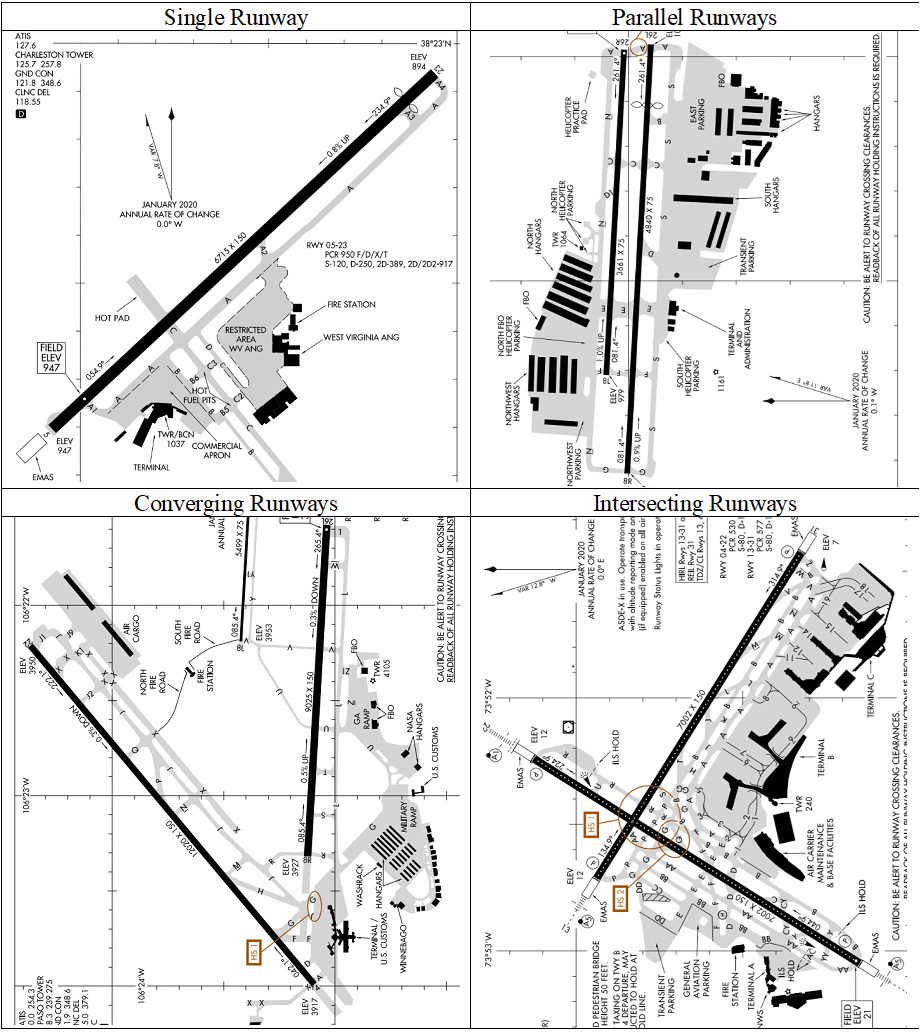
\includegraphics[width = 0.5\textwidth]{Kapitel/runway geometries.png}
    \caption{Runway geometries.}
    \label{fig:enter-label}
\end{figure}

Figure ----- shows 4 types of runway geometries. Single runways are those that do not have any other runway in its vicinity. They can be the only runway in an airport or can be present in airports with multiple runways but with such a separation between them that it can be considered single. Parallel runways are those that run parallel next to each other. Intersecting runways are those that intersect with each other. The angle of the intersection was not considered to be relevant for this project. Converging runways are those that do not physically intersect but whose projections do.

\underline {Type of incident:}
Type of incident describes the cause of the incident by identifying the party at fault. For this project, the type of incidents are differentiated by the following types:

Operational error: An incident caused by the instructions given by the party responsible for ground or aerial traffic control. These incidents can have various causes such as: forgetting previous instructions, failing to communicate instructions, a flawed perception of the current traffic or occupancy of a runway or other human errors.

Pilot deviation: An incident caused when a pilot does not follow instructions, deviates from an approved route and conflicts with other aircraft. These incidents can be caused by poor/lack off communication, confusion or other human errors.

Vehicle deviation: An incident caused by the intrusion of a vehicle in an active runway.

\underline {Class/severity of the incident:}
The classification of the incidents is done by its severity. This is achieved by following ICAO's classification of the severity of runway incursions detailed on ICAO's manual of the prevention of runway incursions. Incursions are classified by severity from A-D, "A" being the most severe. Events with insufficient information are classified as "E". Some of the incidents are assigned an ICAO classification by the entity that does the investigation while others are not. This is mostly dependant on the country in which the incursion took place. If an ICAO severity classification was not given, then one is assigned based on the ICAO classification scheme an the information given in the official report. It is also possible to use the RISC (Runway Incursion Severity Classification) calculator software if there is sufficient information on the incursion.

\begin{figure}[H]
    \centering
    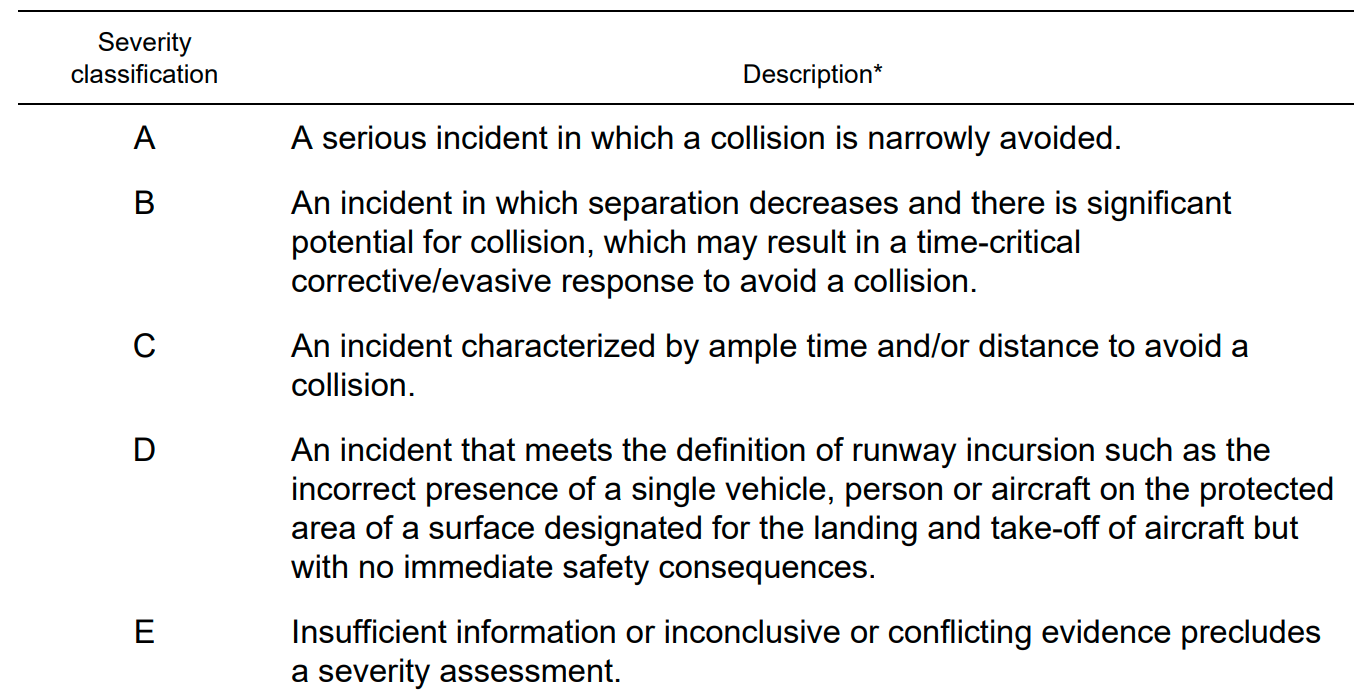
\includegraphics[width = \textwidth]{Kapitel/ICAO Severity classification.png}
    \caption{ICAO runway incursion severity classification scheme}
    \label{fig:enter-label}
\end{figure}

\underline {Model and type of aircrafts involved:} 
This project is mainly concerned with incidents involving commercial or cargo aircrafts. All the incidents that are identified will be added to the data set and they will be categorized by, among other things, the type of aircrafts involved to analyze the incidents.

\underline {OSED states of the aircrafts involved:}
The OSED (Operational Services and Enviromental Definitions) describes the services, functions and procedures for the SURF IA application. It also characterises the enviroment in which it will be used. The OSED states of the aircrafts  derive from this. These OSED States used in DO-323 are the following:

I: Taxiing on Taxiway toward Hold-line or stopped at Holdline.

II: Entering / Crossing / Exiting

III: Takeoff

IV: Approach

V: After Landing

VI: Stopped or taxiing along runway

In the DO-323, These OSED states are used in conjunction with Table A-2 "SURF IA Outputs for all Possible Two-Aircraft State Combinations" to determine which combination of states of the aircrafts involved result in which SURF IA output. In incidents involving pilot deviations, Ownership will be assigned to the aircraft that was following ATC instructions. The aircraft causing the incursion will be the "other aircraft".

\subsection{Sources}
Official websites of organizations investigating aviation accidents and incidents of the following countries were scouted for the reports: Albania, Argentina, Armenia, Australia, Austria, Belgium, Brazil, Bulgaria, Canada, Channel Islands, China, Columbia, Denmark, Estonia, Ethiopia, Finland, France, Germany, Greece, Greenland, Hong Kong, Hungary, Iceland, India, Indonesia, Iran, Italy, Japan, Lithuania, Luxembourg, Malaysia, Mexico, Mongolia, Myanmar, Netherlands, New Zealand, Norway, Peru, Philippines, Poland, Portugal, Republic of Ireland, Russia, Saudi Arabia, Serbia, Singapore, South Africa, South Korea, Spain, Sri Lanka, Sweden, Switzerland, The Bahamas, United Arab Emirates, United Kingdom, United States.

Main and other sources:
\begin{itemize}
    \item FAA Runway incursion database: \url{https://www.asias.faa.gov/apex/f?p=100:5:::NO}
    \item NTSB investigation reports: \url{https://www.ntsb.gov/investigations/AccidentReports/Pages/Reports.aspx}
    \item Aviation Safety Network: \url{https://asn.flightsafety.org/database/}
    \item Bundesstelle für Flugunfalluntersuchung: \url{https://www.bfuweb.de/DE/Publikationen/OpenData/opendata_node.html}
    \item Skybrary: \url{https://skybrary.aero/operational-issues/runway-incursion}
    \item Australia ATSB aviation investigations: \url{https://www.atsb.gov.au/aviation-investigation-reports}
    \item ICAO runway safety statistics: \url{https://www.icao.int/Aerodromes/RunwaySafety/Pages/Statistics.aspx}
\end{itemize}


\subsection{Data Categorization}

After identifying the runway incursions that took place after 1995, extracting the data and adding it to the data set, it is possible to categorize the information to  analyze it and draw useful conclusions. This is a necessary step as not all of the runway incursions that were identified and included in the data set are of part of the main focus of this project. This might because of the type of aircrafts that were involved, the severity of the incident or due to lack of information.

The raw number of incidents identified was 33133, 32898 coming from the FAA. This is because the reporting culture of runway incursion incidents varies from country to country. The FAA lists all of the incidents that are identified, assigns them an ICAO classification and includes them in their database. Other countries don't do this and while reports and investigations are done, it is not done in the same manner as in the United states. That said, severe cases are rare. Events that fit the ICAO classification of "C" and "D" make up the majority of the incursions that take place. To reduce the number of entries that are not the main focus of this project on the data set, FAA incursions of severity "C" and "D" will not be included in the data set. Incursions with incomplete data and those whose cause is listed as "other" will also be omitted. Doing this, the number of runway incursions incidents in the data set is reduced to 484 globally.

\begin{figure}[H]
    \centering
    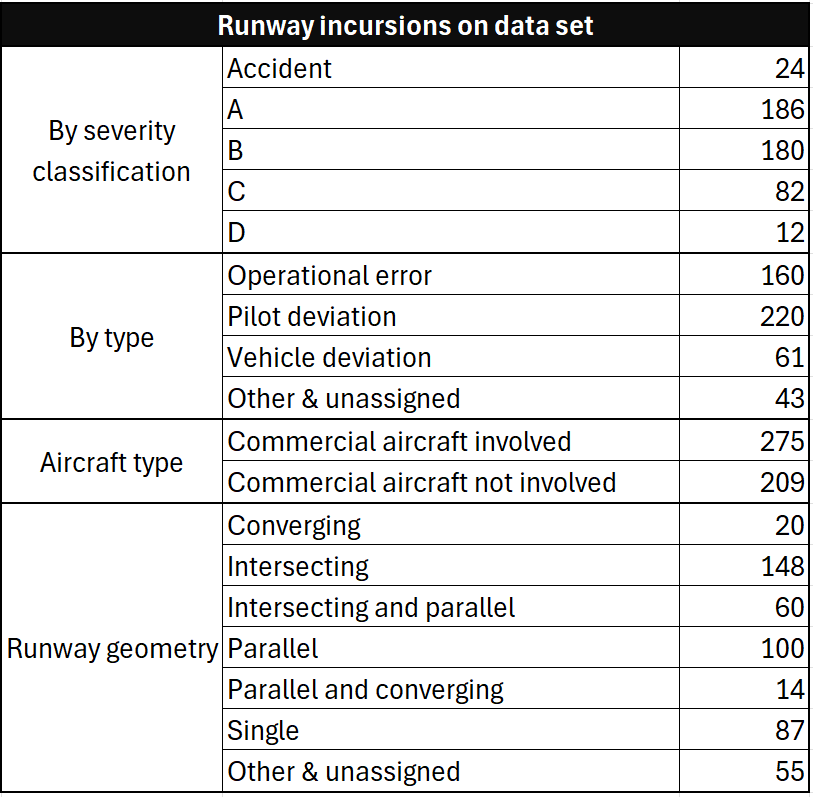
\includegraphics[width = 0.5\textwidth]{Kapitel/Runway incursion full data set classified.png}
    \caption{Classification of data set by different parameters}
    \label{fig:enter-label}
\end{figure}

Figure ---- shows a summary of the full data set. The incidents there are classified by their severity, type, aircraft type and runway geometry. The severity of the incident and the involvement of a commercial aircraft will be used to determine whether the entries are relevant to the main focus of this project.

With the number of entries reduced, the focus shifts to identifying the incidents that are relevant to the main focus of this project, which is severe incidents and accidents involving commercial aircrafts. A distinction will be made between incidents that involve two aircrafts, with at least one of them being commercial, and incidents that involve a ground vehicle and a commercial aircraft. The number of incidents of classification "A" and "B" involving a commercial aircraft is 151. The number of incidents that involve a commercial aircraft and a vehicle is 40. Thus, 191 incidents are found to be relevant for this project.

\subsection{Difference between Data Collected and Data used by SURF IA}

Data collected is conflict geometry, runway geometry, uses severity of outcome based framework. ICAO RIS category based on RISC calculator.

SURF IA uses aircraft states, directionality, speed and calculates a convergence rate to determine if separation will pose safety hazard. In effect, it is calculating a potential collision risk. Uses risk based framework.

to adapt data used, accident reports are read to determine aircraft OSA state in accordance with do323, method of calculating convergence rate is not listed in rtca do 323, just timing thresholds for alerts. 

\subsection{Data Verification}

Collected data severity category was verified using ICAO RISC calculator. faa provides severity levels


\section{Analysis}

\subsection{Alert}
\chapter{Results}
\label{ch:grundlagen}

Wichtige Info: Als Compiler muss \textbf{LuaLaTeX} verwendet werden. Auch in ShareLatex!

\section{Effectiveness Analysis}

[reword later]

is SURF IA less effective on certain runway geometries or not?

is SURF 
\section{Runway Incursions Distribution}
After thorough analysis of collected data, it was discovered, that vast majority of reported Runway Incursions happens in the United States (figure 4.1). Such strong concentration, might be due to cultural differences between countries on a topic of incident reporting. Relevant cases are shown on figure 4.2

\begin{figure} [H]
    \centering
    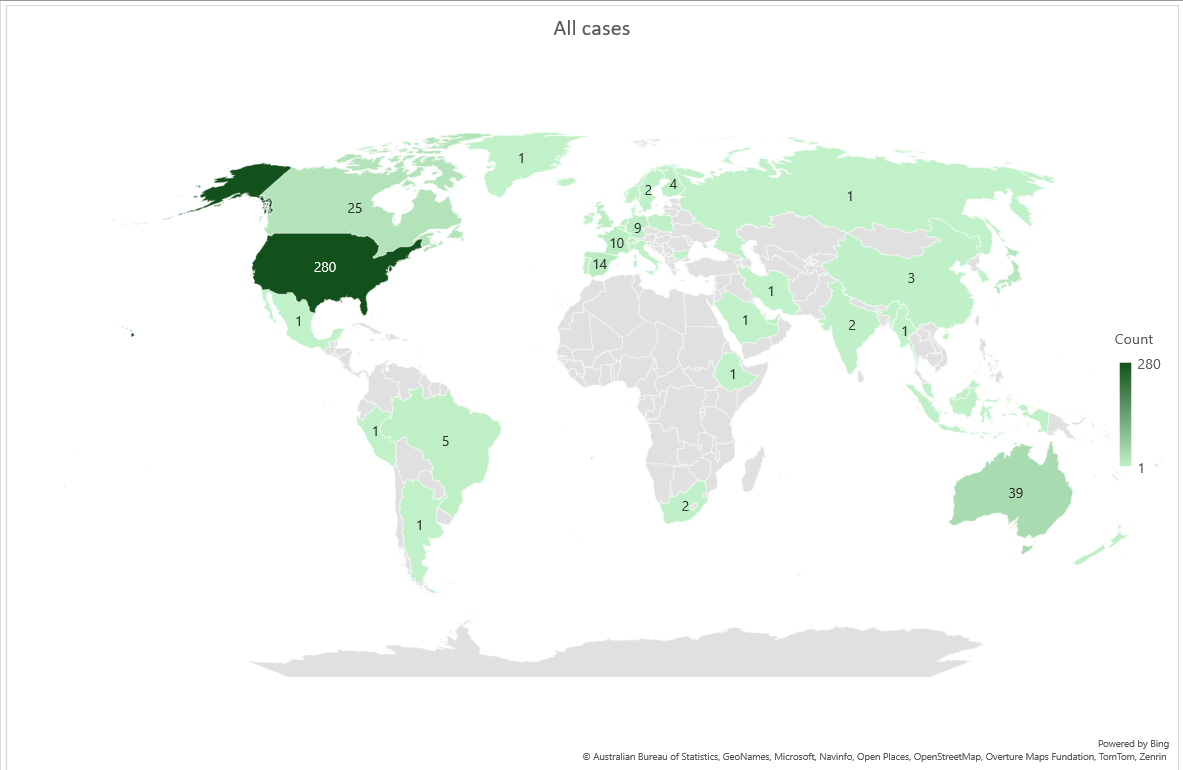
\includegraphics[width=0.9\linewidth]{Abbildungen/Geo_All.png}
    \caption{Geography of all incidents and accidents}
    \label{fig:enter-label}
\end{figure}

\begin{figure} [H]
    \centering
    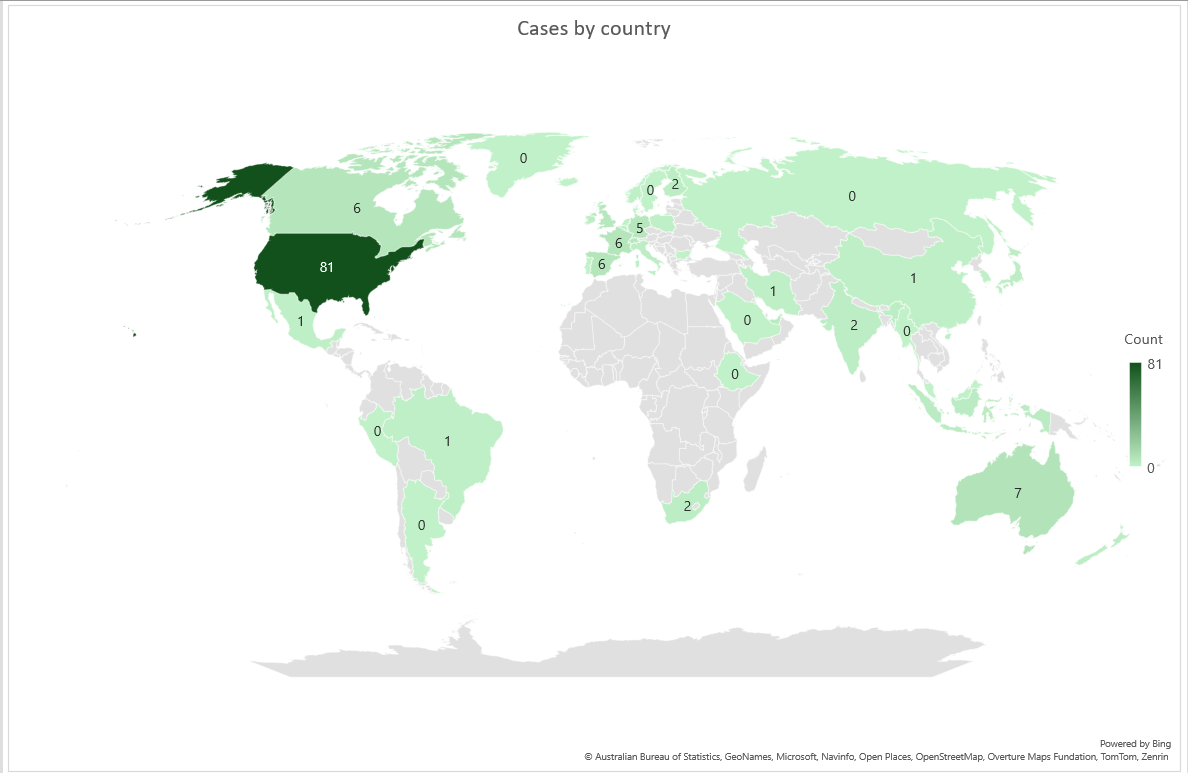
\includegraphics[width=0.9\linewidth]{Abbildungen/Geo_Relevant.png}
    \caption{Geography of relevant incidents and accidents}
    \label{fig:enter-label}
\end{figure}

 
\section{Analysis of Runway Incursions} 
It was discovered, that there are similar trends in runway incursions for both commercial and general aviation (figure 4.2). Although, it must be said, that the number of commercial cases in reality is higher, and number of cases is reduced due to strict filters for relevant cases for commercial aviation.

\begin{figure} [H]
        \centering
        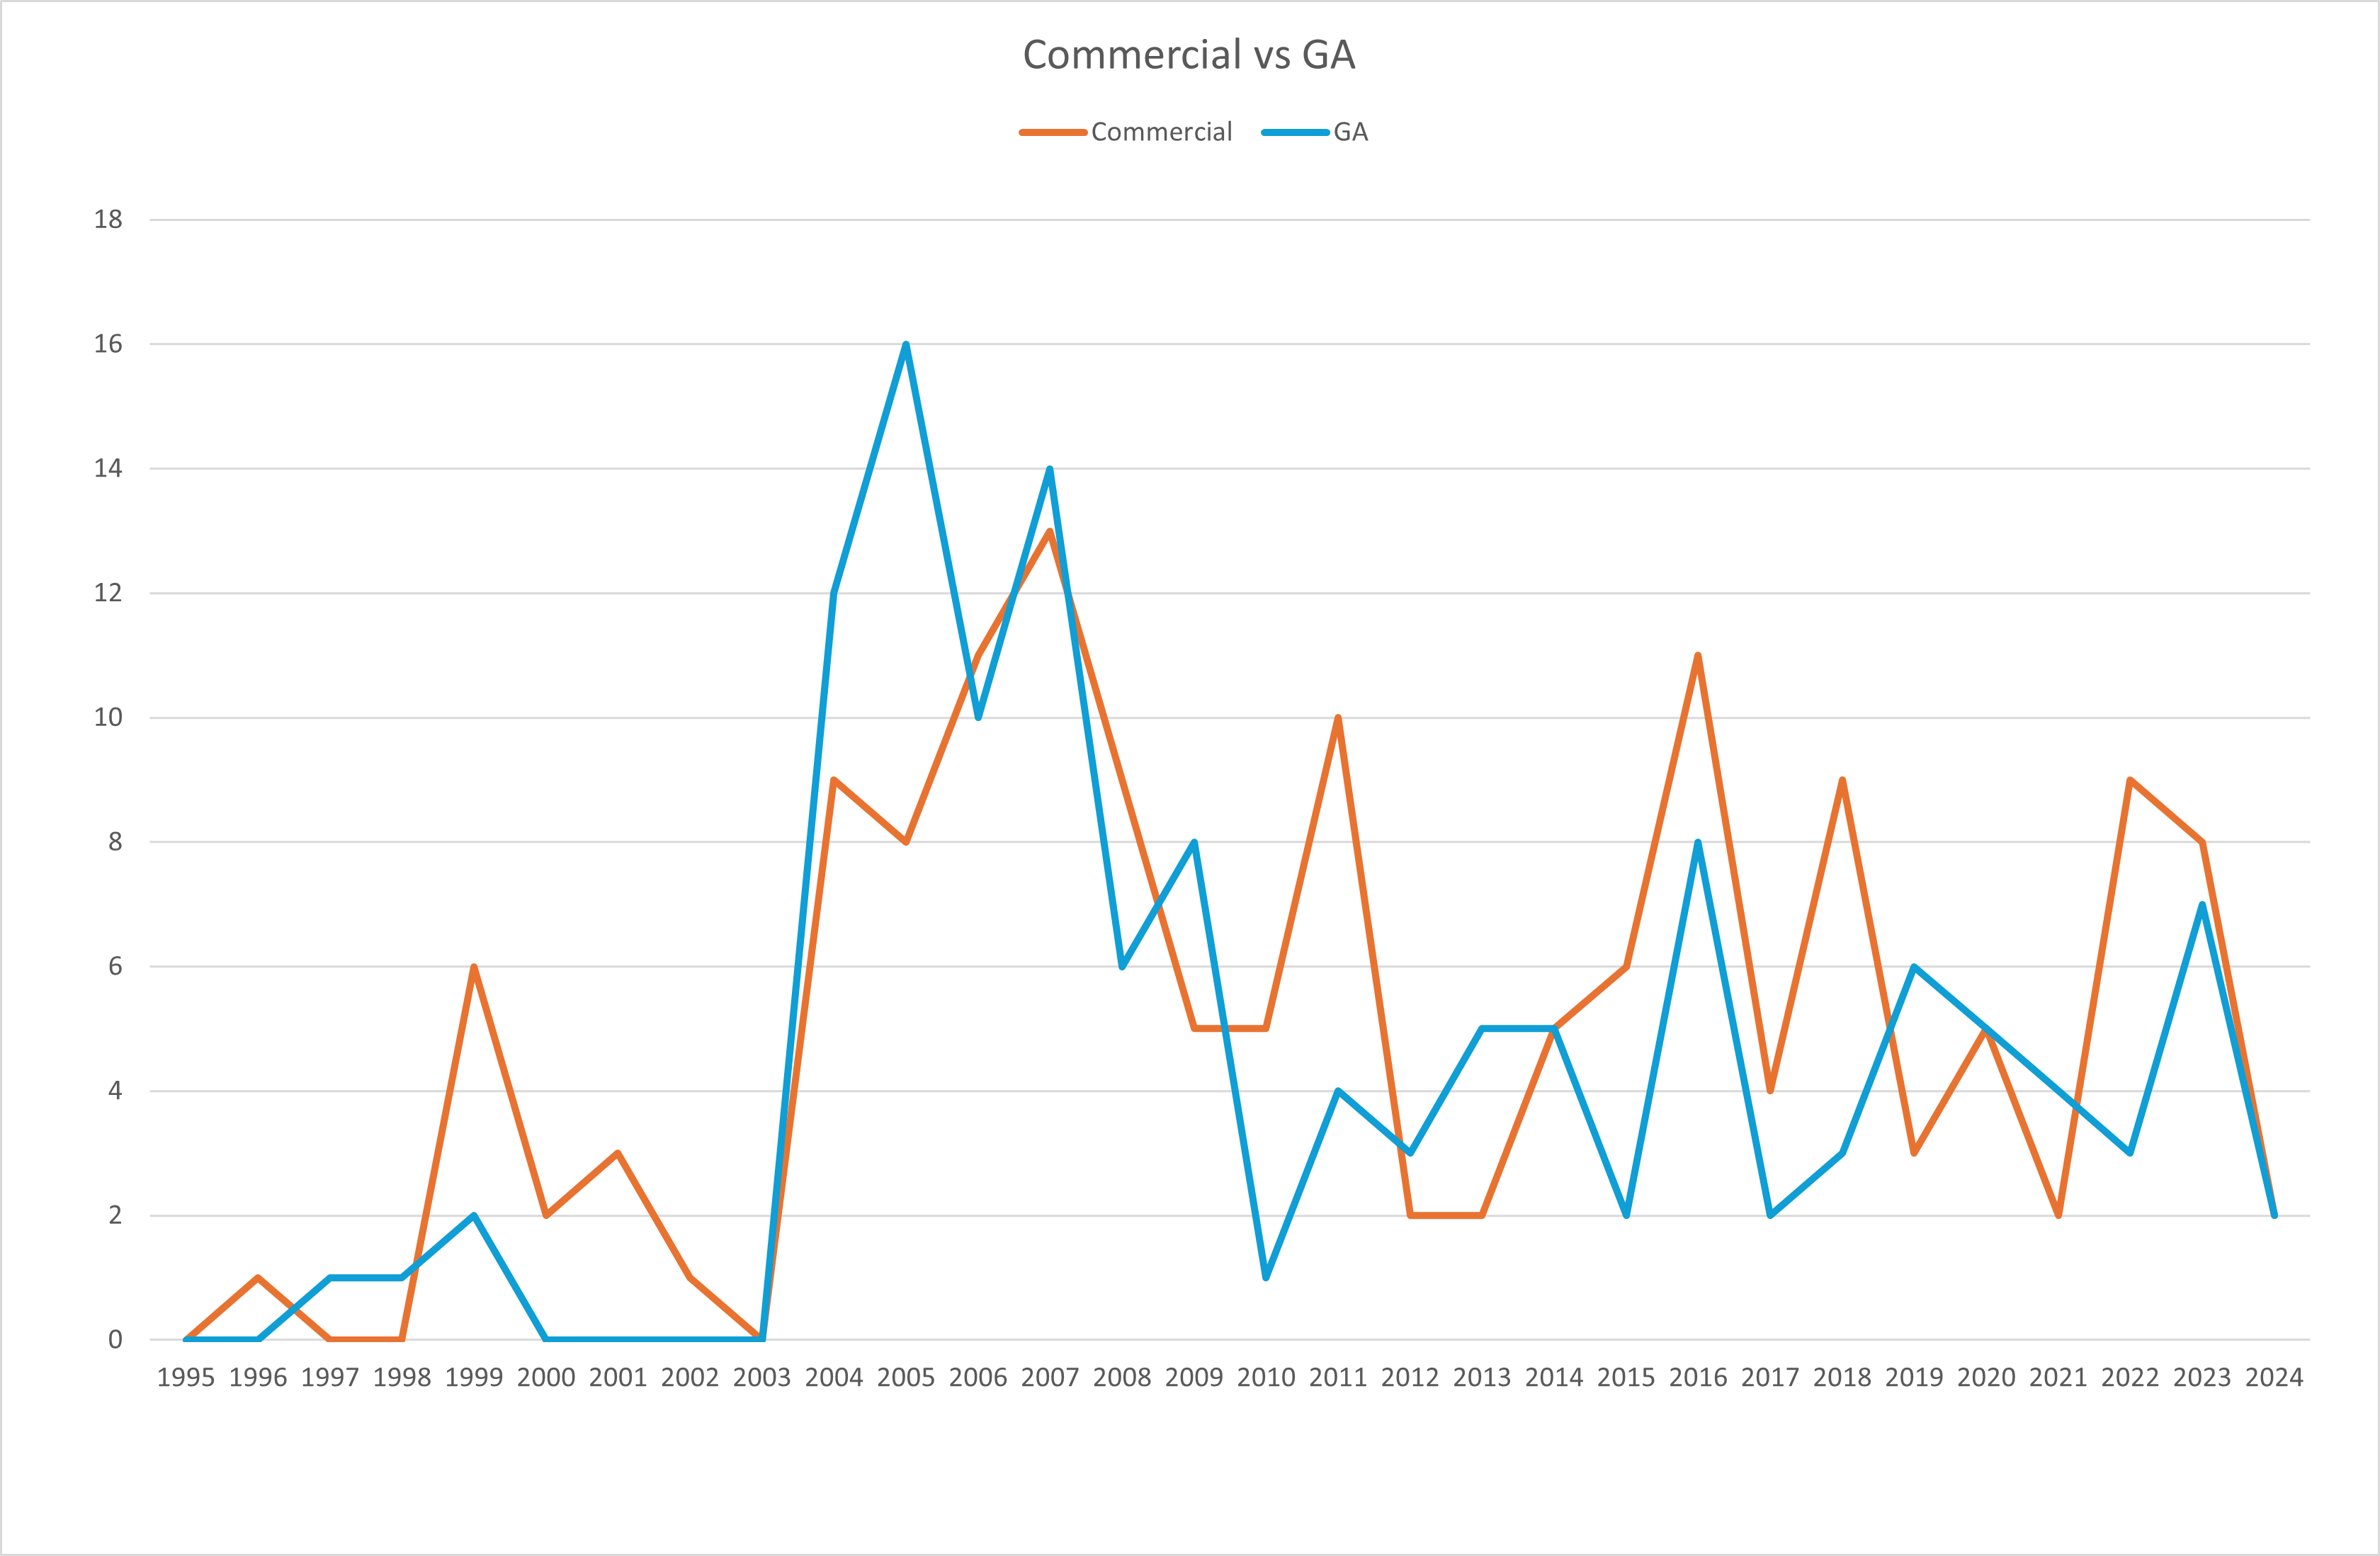
\includegraphics[width=0.75\linewidth]{Commercial_vs_GA_year.png}
        \caption{Commercial and GA year by year}
        \label{fig:enter-label}
\end{figure}


show frequency distribution graphs of category a and b runway incursions and effectiveness of SURF vs different parameters (runway geometry, cause, ownship and target type?. runway geometry for sure, still need to discuss about other parameters) discuss. try to find SURF detection logic reasoning for less effective detections vs others regarding conflict geometry

More than a half of the incidents were caused due to ATC error, or Operational Error (OE). While the other half was caused by Pilot Deviation (PD) or Pedestrian/Vehicle Deviation (P/VD).
\begin{figure} [H]
    \centering
    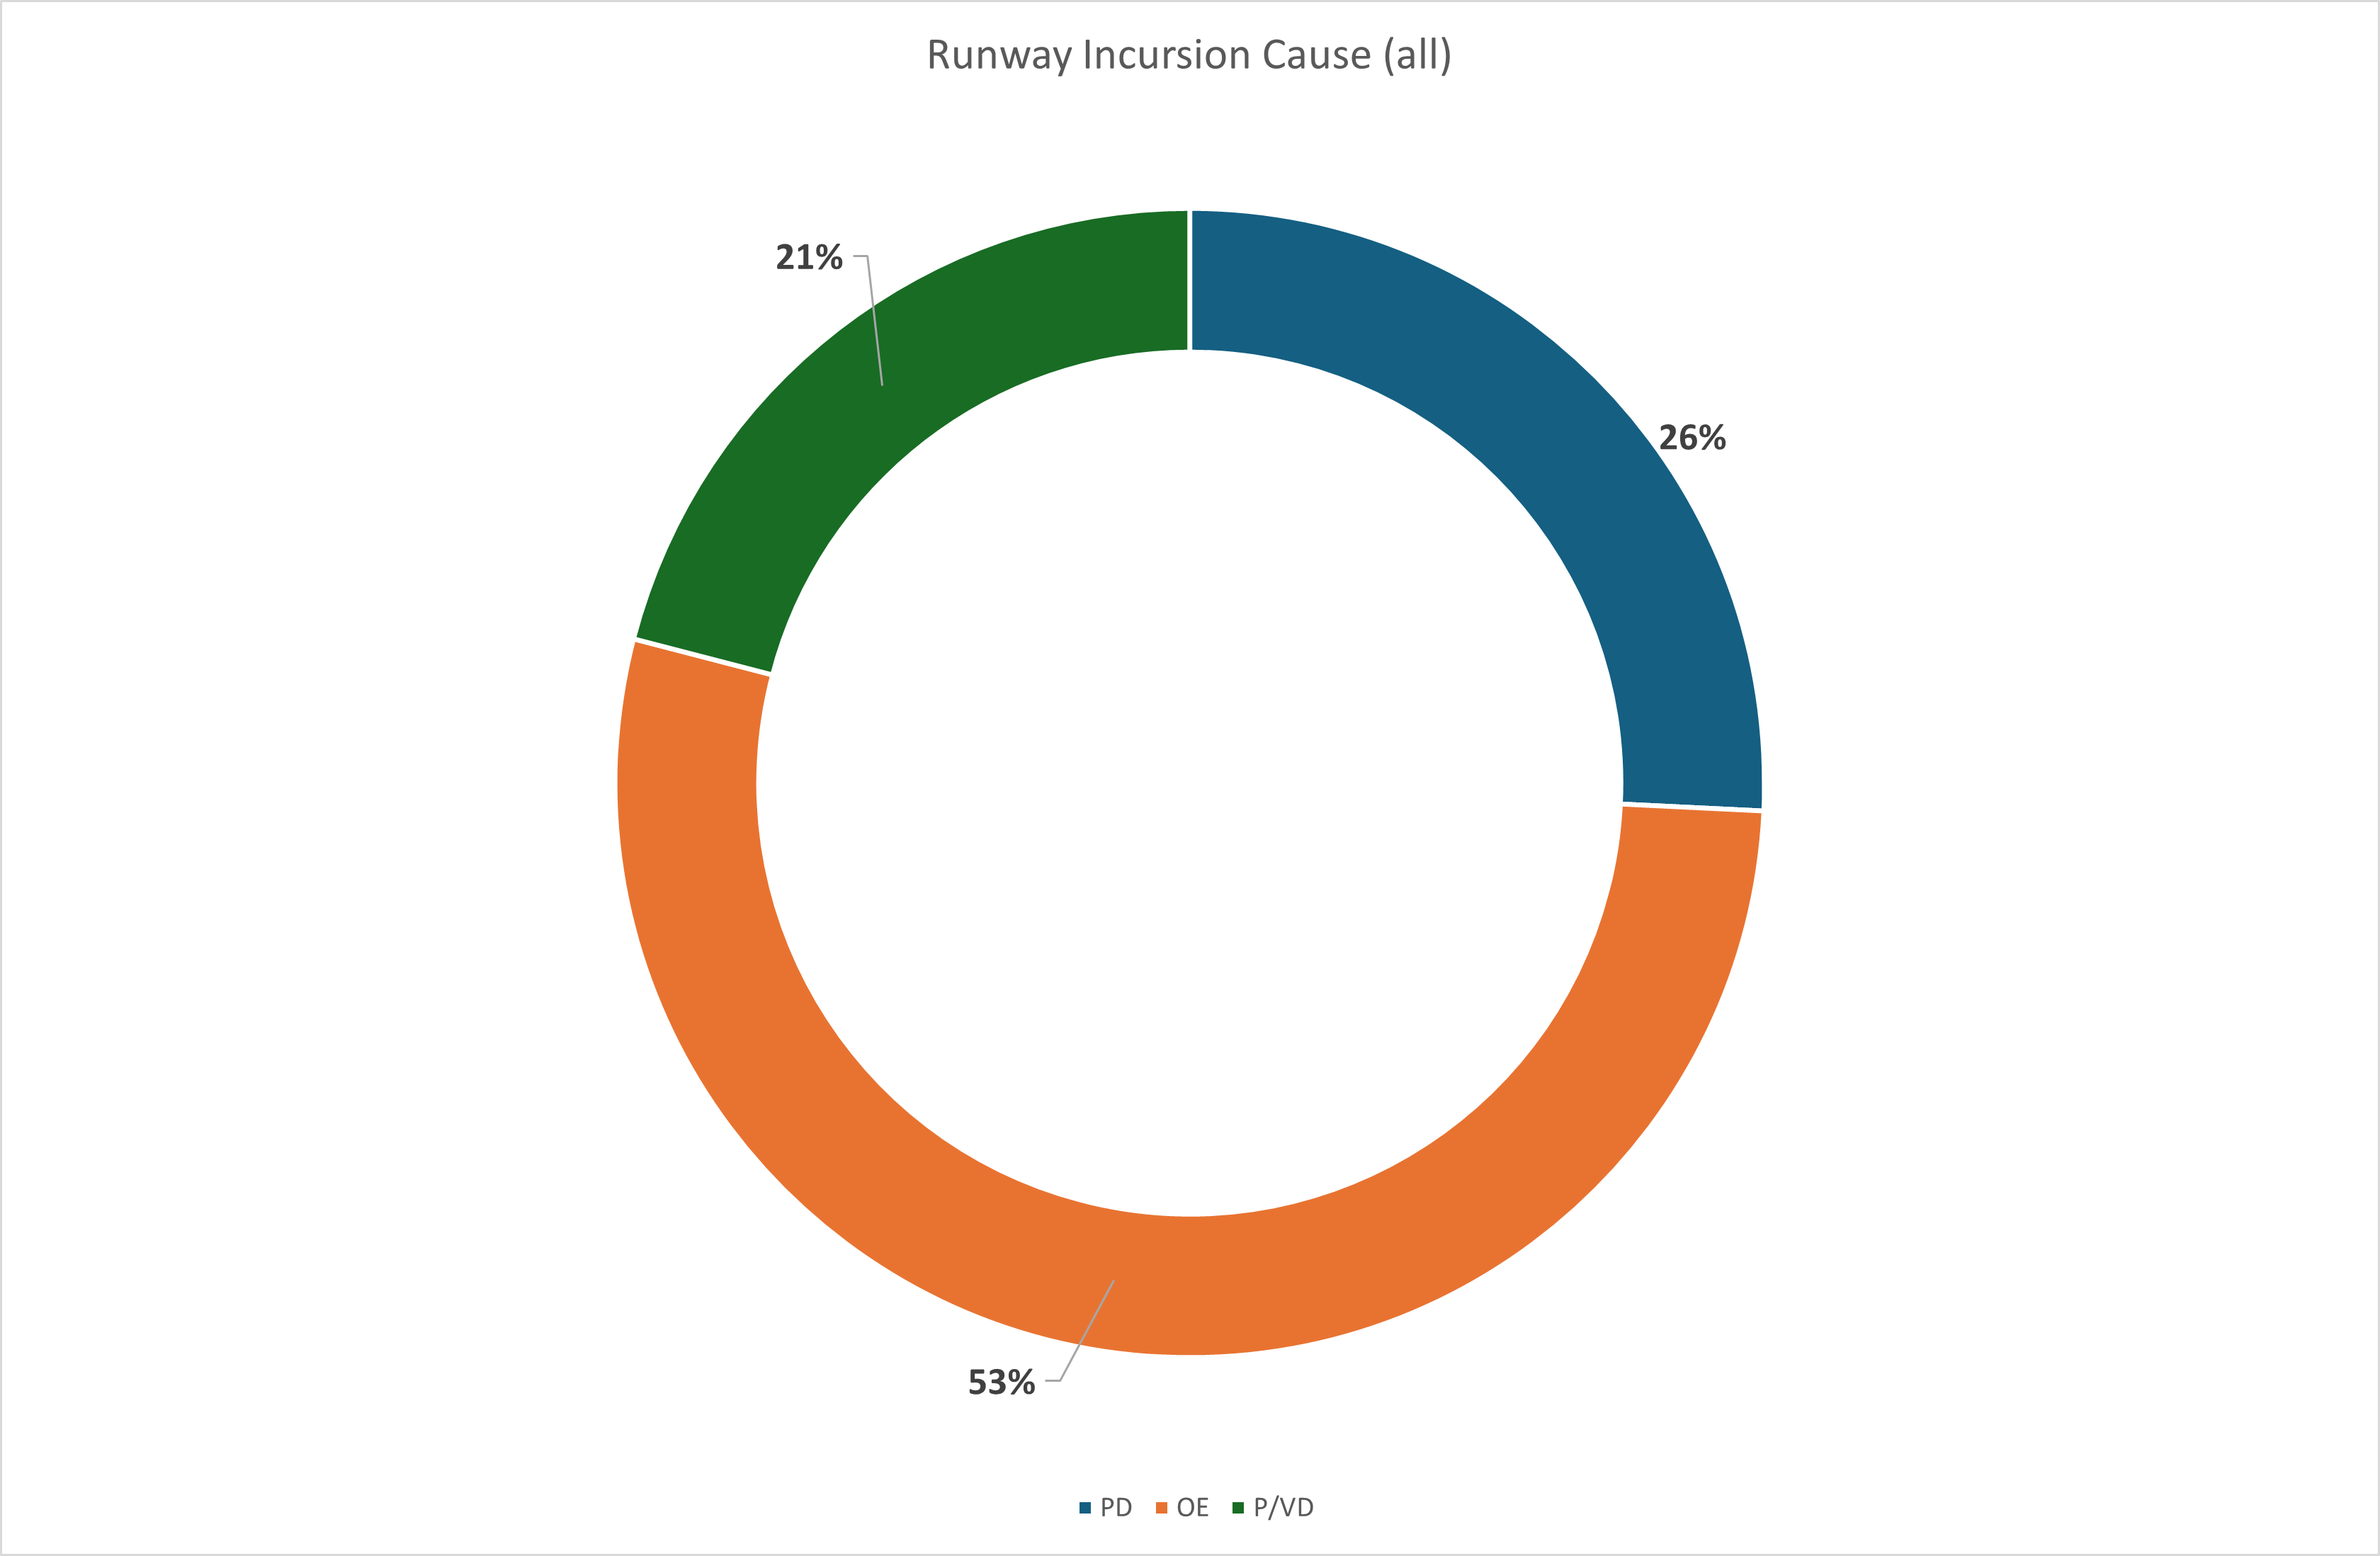
\includegraphics[width=0.75\linewidth]{Abbildungen/Cause_All.png}
    \caption{Cause All}
    \label{fig:enter-label}
\end{figure}

While in cases, that adhere to provided parameters - proportion is roughly 1 to 1 between PD and OE.
\begin{figure} [H]
    \centering
    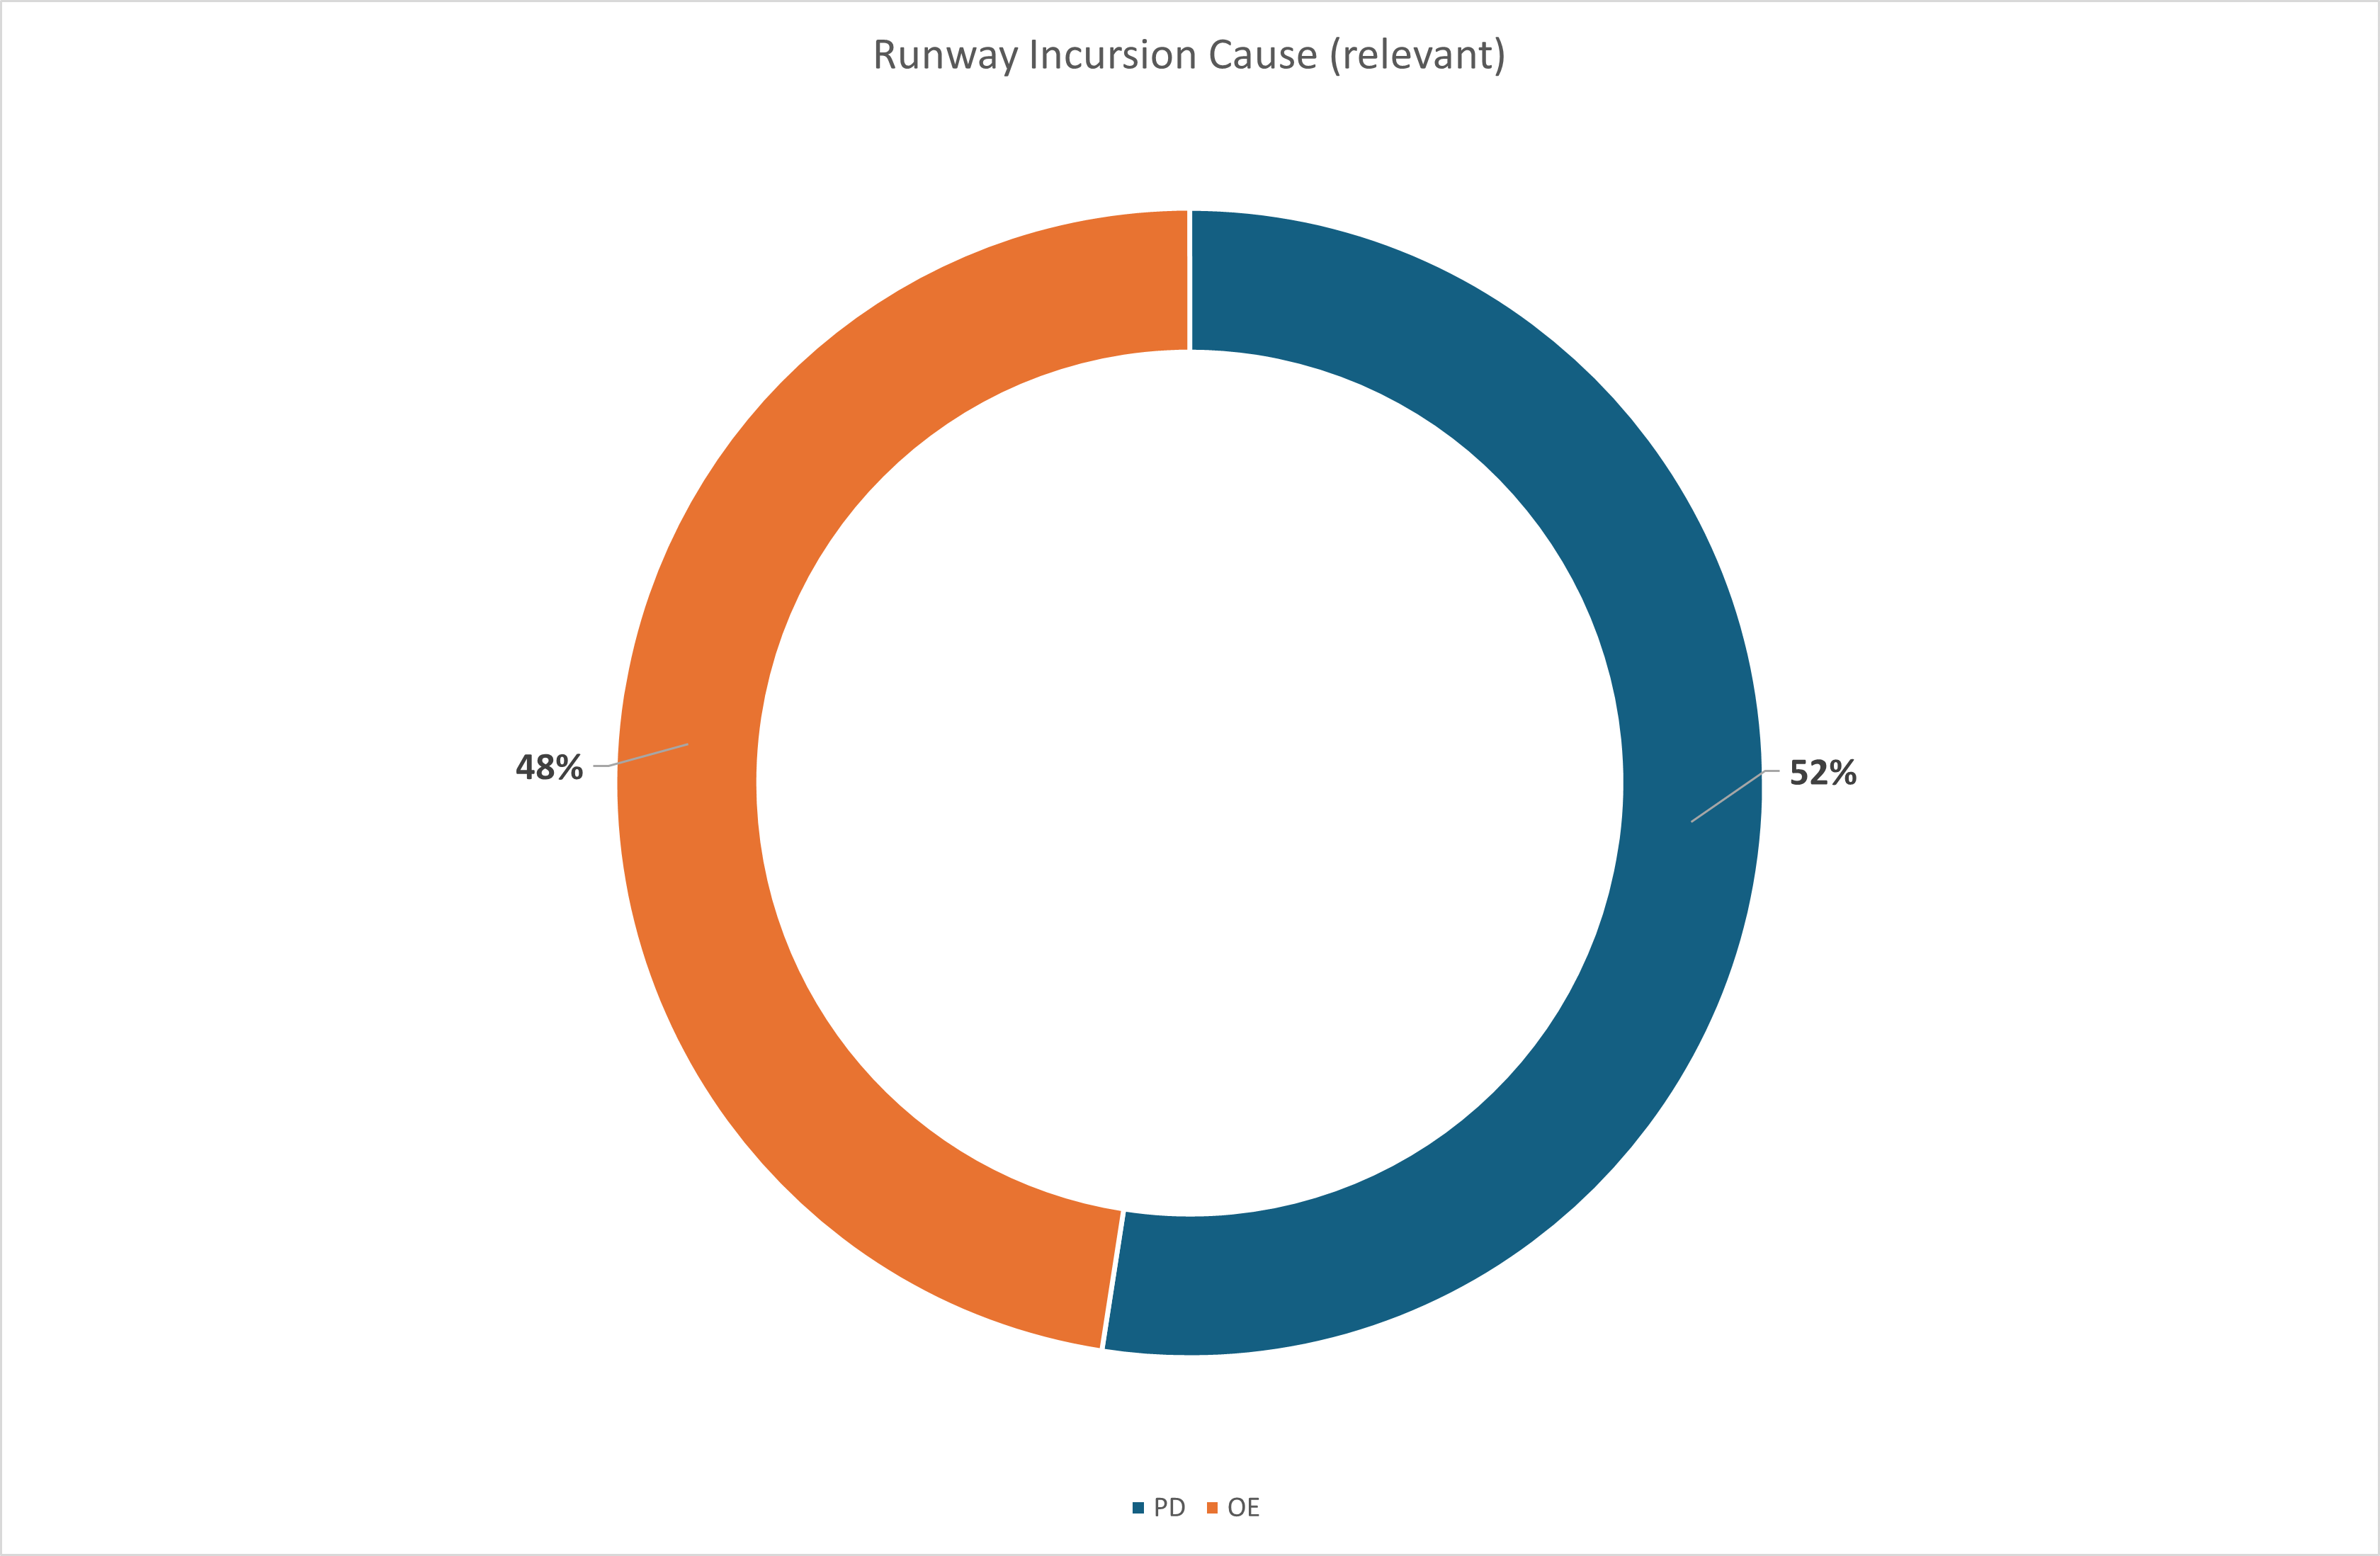
\includegraphics[width=0.75\linewidth]{Abbildungen/Cause_relevant.png}
    \caption{Cause Relevant}
    \label{fig:enter-label}
\end{figure}

\begin{figure} [H]
    \centering
    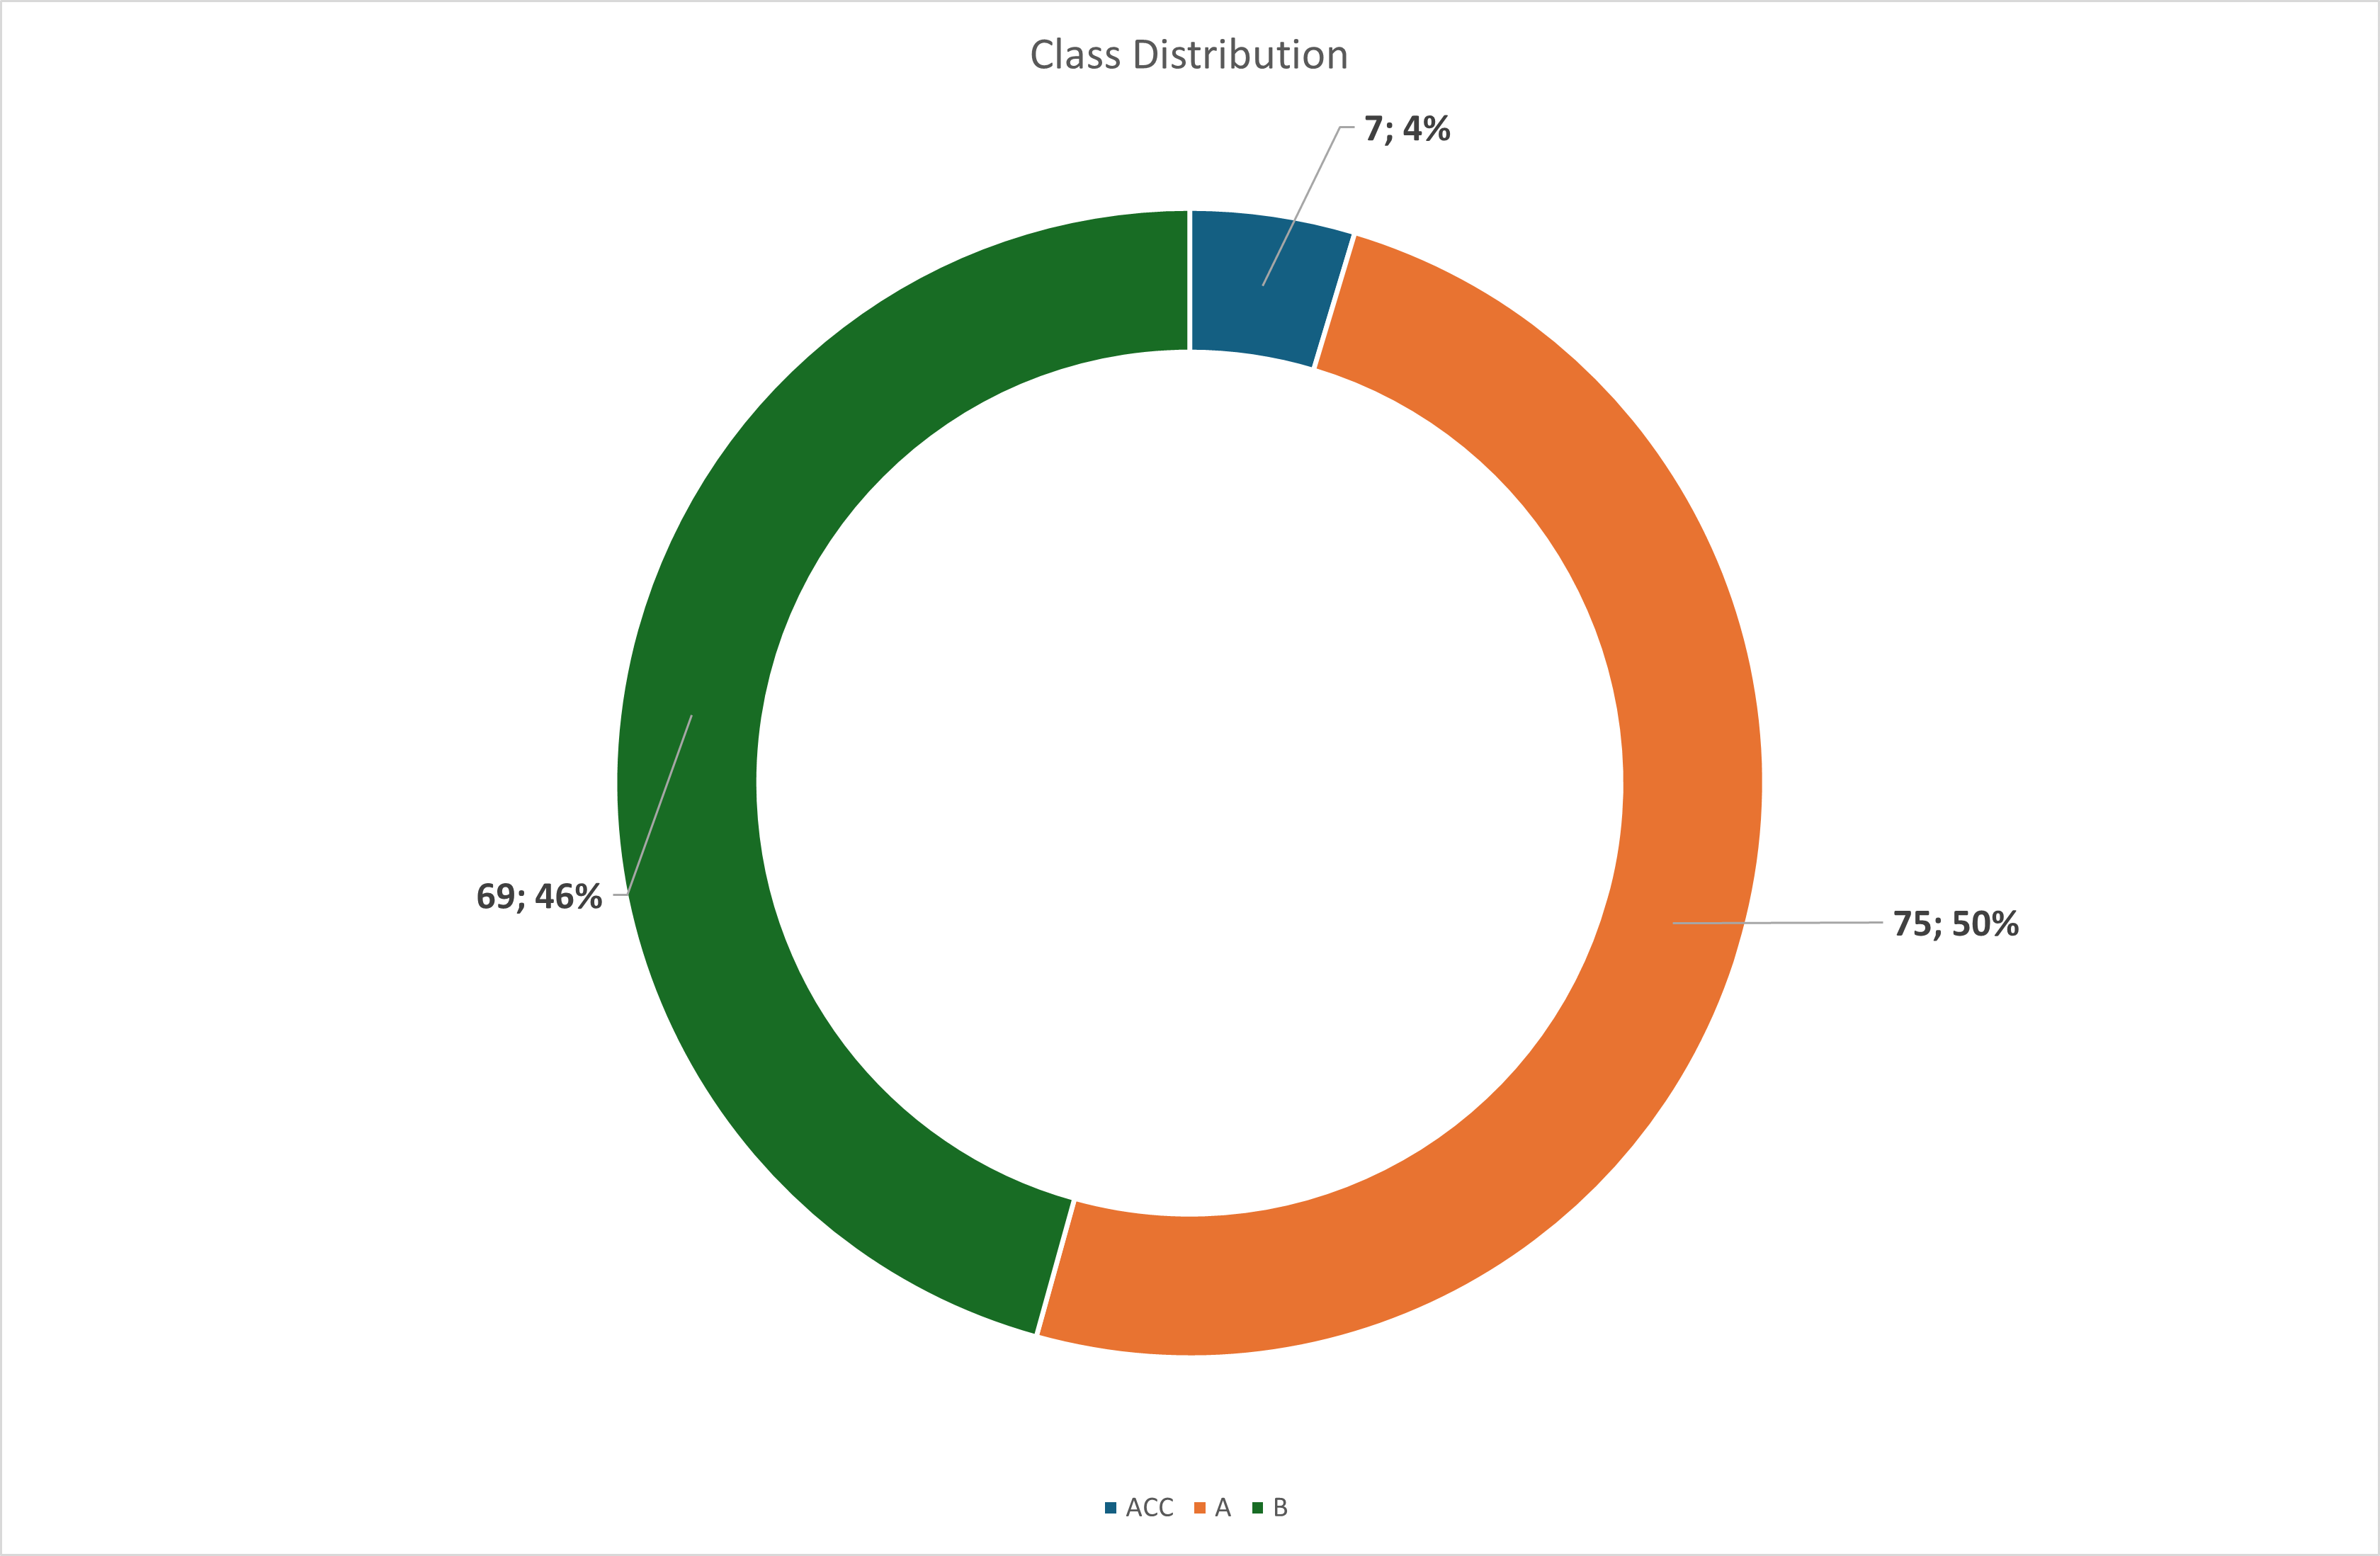
\includegraphics[width=0.75\linewidth]{Abbildungen/Class_relevant.png}
    \caption{Class Distribution}
    \label{fig:enter-label}
\end{figure}

The number of relevant cases was reduced to 192. 151 incidents involving two aircrafts, of which at least one is commercial, and the rest involving one commercial aircraft and a ground vehicle.

\subsection{A and B Runway incursions involving a commercial aircraft}

\begin{figure}[H]
    \centering
    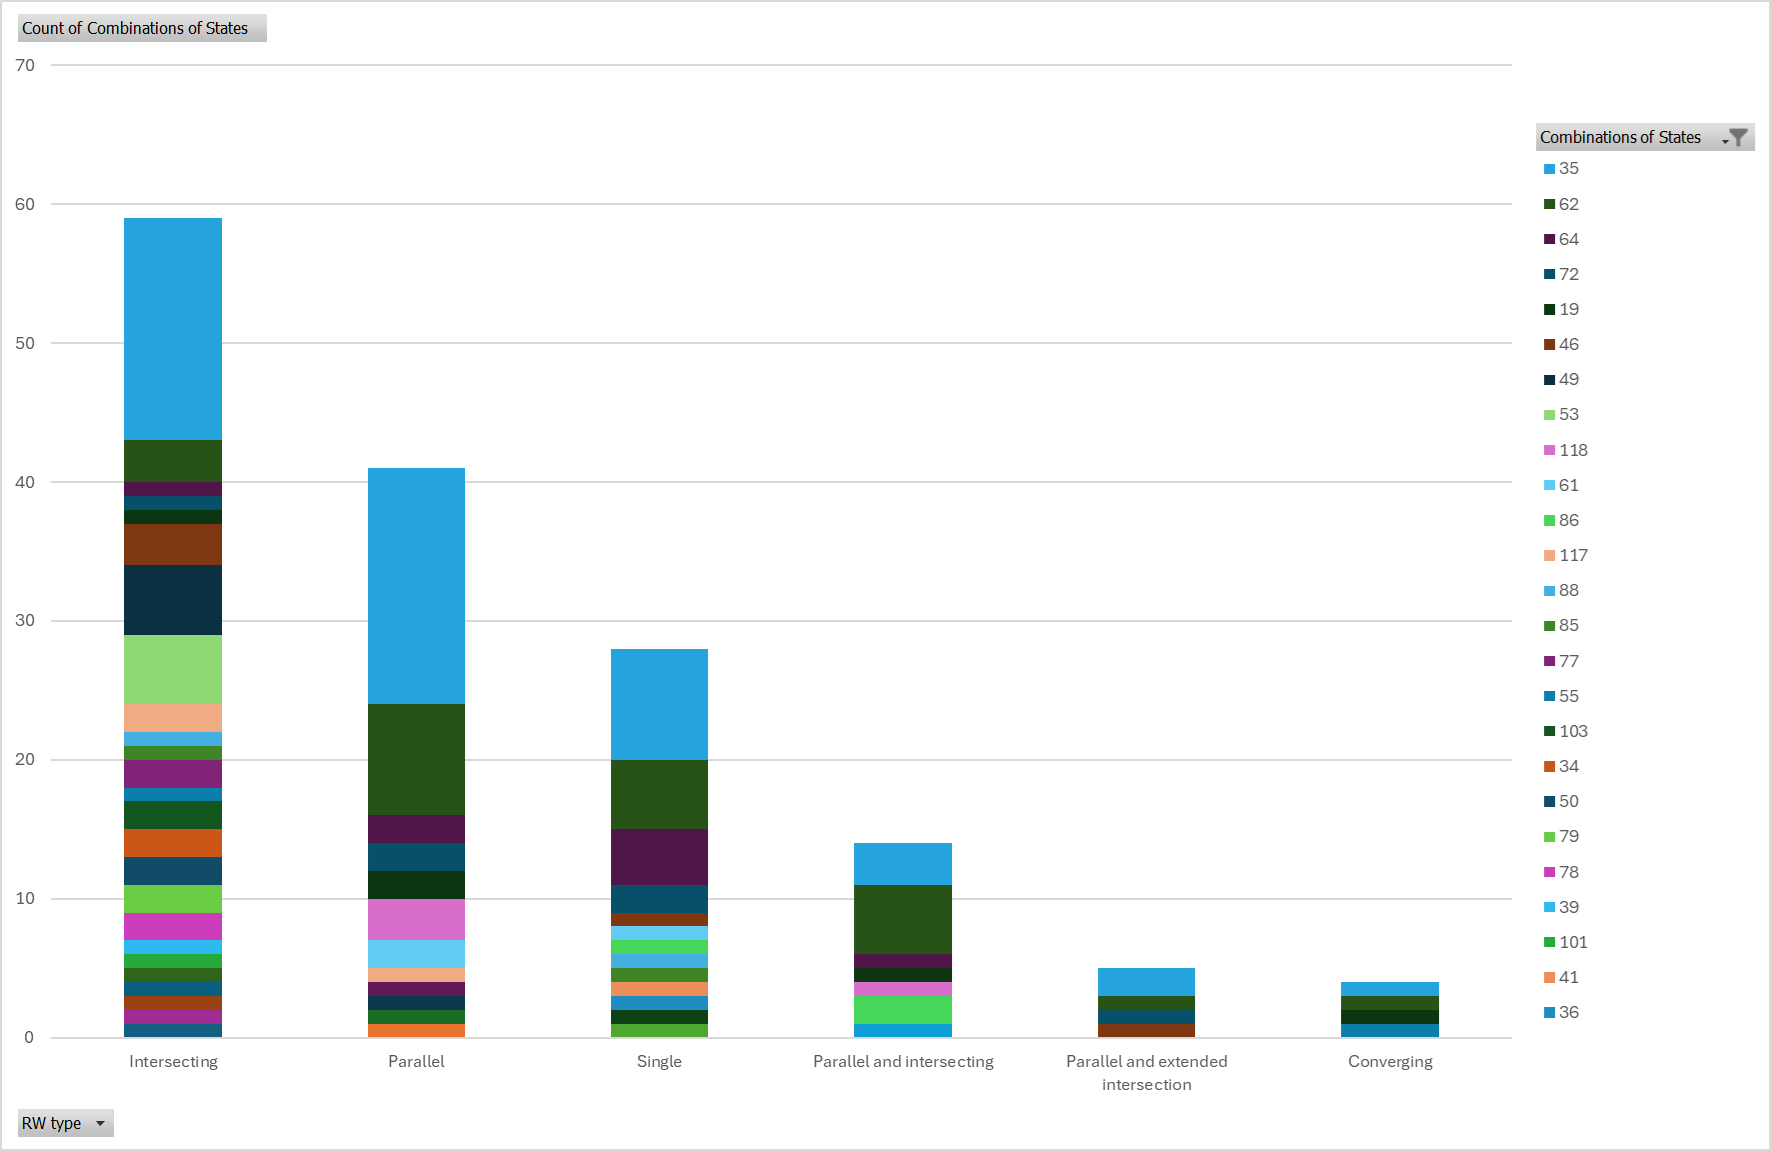
\includegraphics[width = 1\textwidth]{Kapitel/Commercial x other - incursions by runway geometry.png}
    \caption{Count of incidents of A and B Severity involving a commercial aircraft}
    \label{fig:enter-label}
\end{figure}

Figure --- shows the combination of states of the 151 relevant incidents by runway geometry. The runway geometry that has the most incursion cases is the intersecting runway layout, with a total of 59 relevant incidents. It is followed by parallel and single runways, with 41 and 28 incidents respectively. It can be observed that the most common combinations of states are prevalent in every type of runway geometry. 

\begin{table}[H]
\begin{tabular}{cccc}
Combination of   states & Number of runway incursions & ACFT 1 OSED & ACFT 2 OSED \\
35                      & 46                          & III         & II          \\
62                      & 22                          & IV          & II          \\
64                      & 8                           & IV          & III         \\
72                      & 6                           & IV          & VI          \\
46                      & 5                           & III         & VI          \\
49                      & 5                           & III         & IV          \\
53                      & 5                           & III         & III         \\
19                      & 4                           & II          & III         \\
118                     & 4                           & VI          & IV          \\
61                      & 3                           & IV          & I           \\
86                      & 3                           & V           & II          \\
117                     & 3                           & VI          & IV          \\
34                      & 2                           & III         & I           \\
50                      & 2                           & III         & IV          \\
77                      & 2                           & IV          & III         \\
78                      & 2                           & IV          & III         \\
79                      & 2                           & IV          & VI          \\
85                      & 2                           & V           & I           \\
88                      & 2                           & V           & III         \\
103                     & 2                           & V           & III         \\
1                       & 1                           & I           & I           \\
6                       & 1                           & I           & V           \\
21                      & 1                           & II          & IV          \\
36                      & 1                           & III         & II          \\
39                      & 1                           & III         & III         \\
41                      & 1                           & III         & IV          \\
54                      & 1                           & III         & III         \\
55                      & 1                           & III         & VI          \\
56                      & 1                           & III         & VI          \\
74                      & 1                           & IV          & IV          \\
97                      & 1                           & V           & VI          \\
98                      & 1                           & V           & VI          \\
101                     & 1                           & V           & V           \\
111                     & 1                           & VI          & I           \\
112                     & 1                           & VI          & II          \\
116                     & 1                           & VI          & III         \\
130                     & 1                           & VI          & III         \end{tabular}
    \caption{Runway incursions by combination of states} 
\end{table}

Table --- lists the combination of states obtained and the number of incursions that each of those combinations have. combinations of states 35 and 62 are the most common ones, adding up to 68 incursions. 
Those combinations resemble one another in the OSED state of the second aircraft, which is II. this corresponds to events in which the second aircraft enters or crosses the runway while it is being used. If we add combinations 86, 36, and 112, which also involve a second aircraft entering the occupied runway, the number of incursions rises to 73. 


\begin{figure}[H]
    \centering
    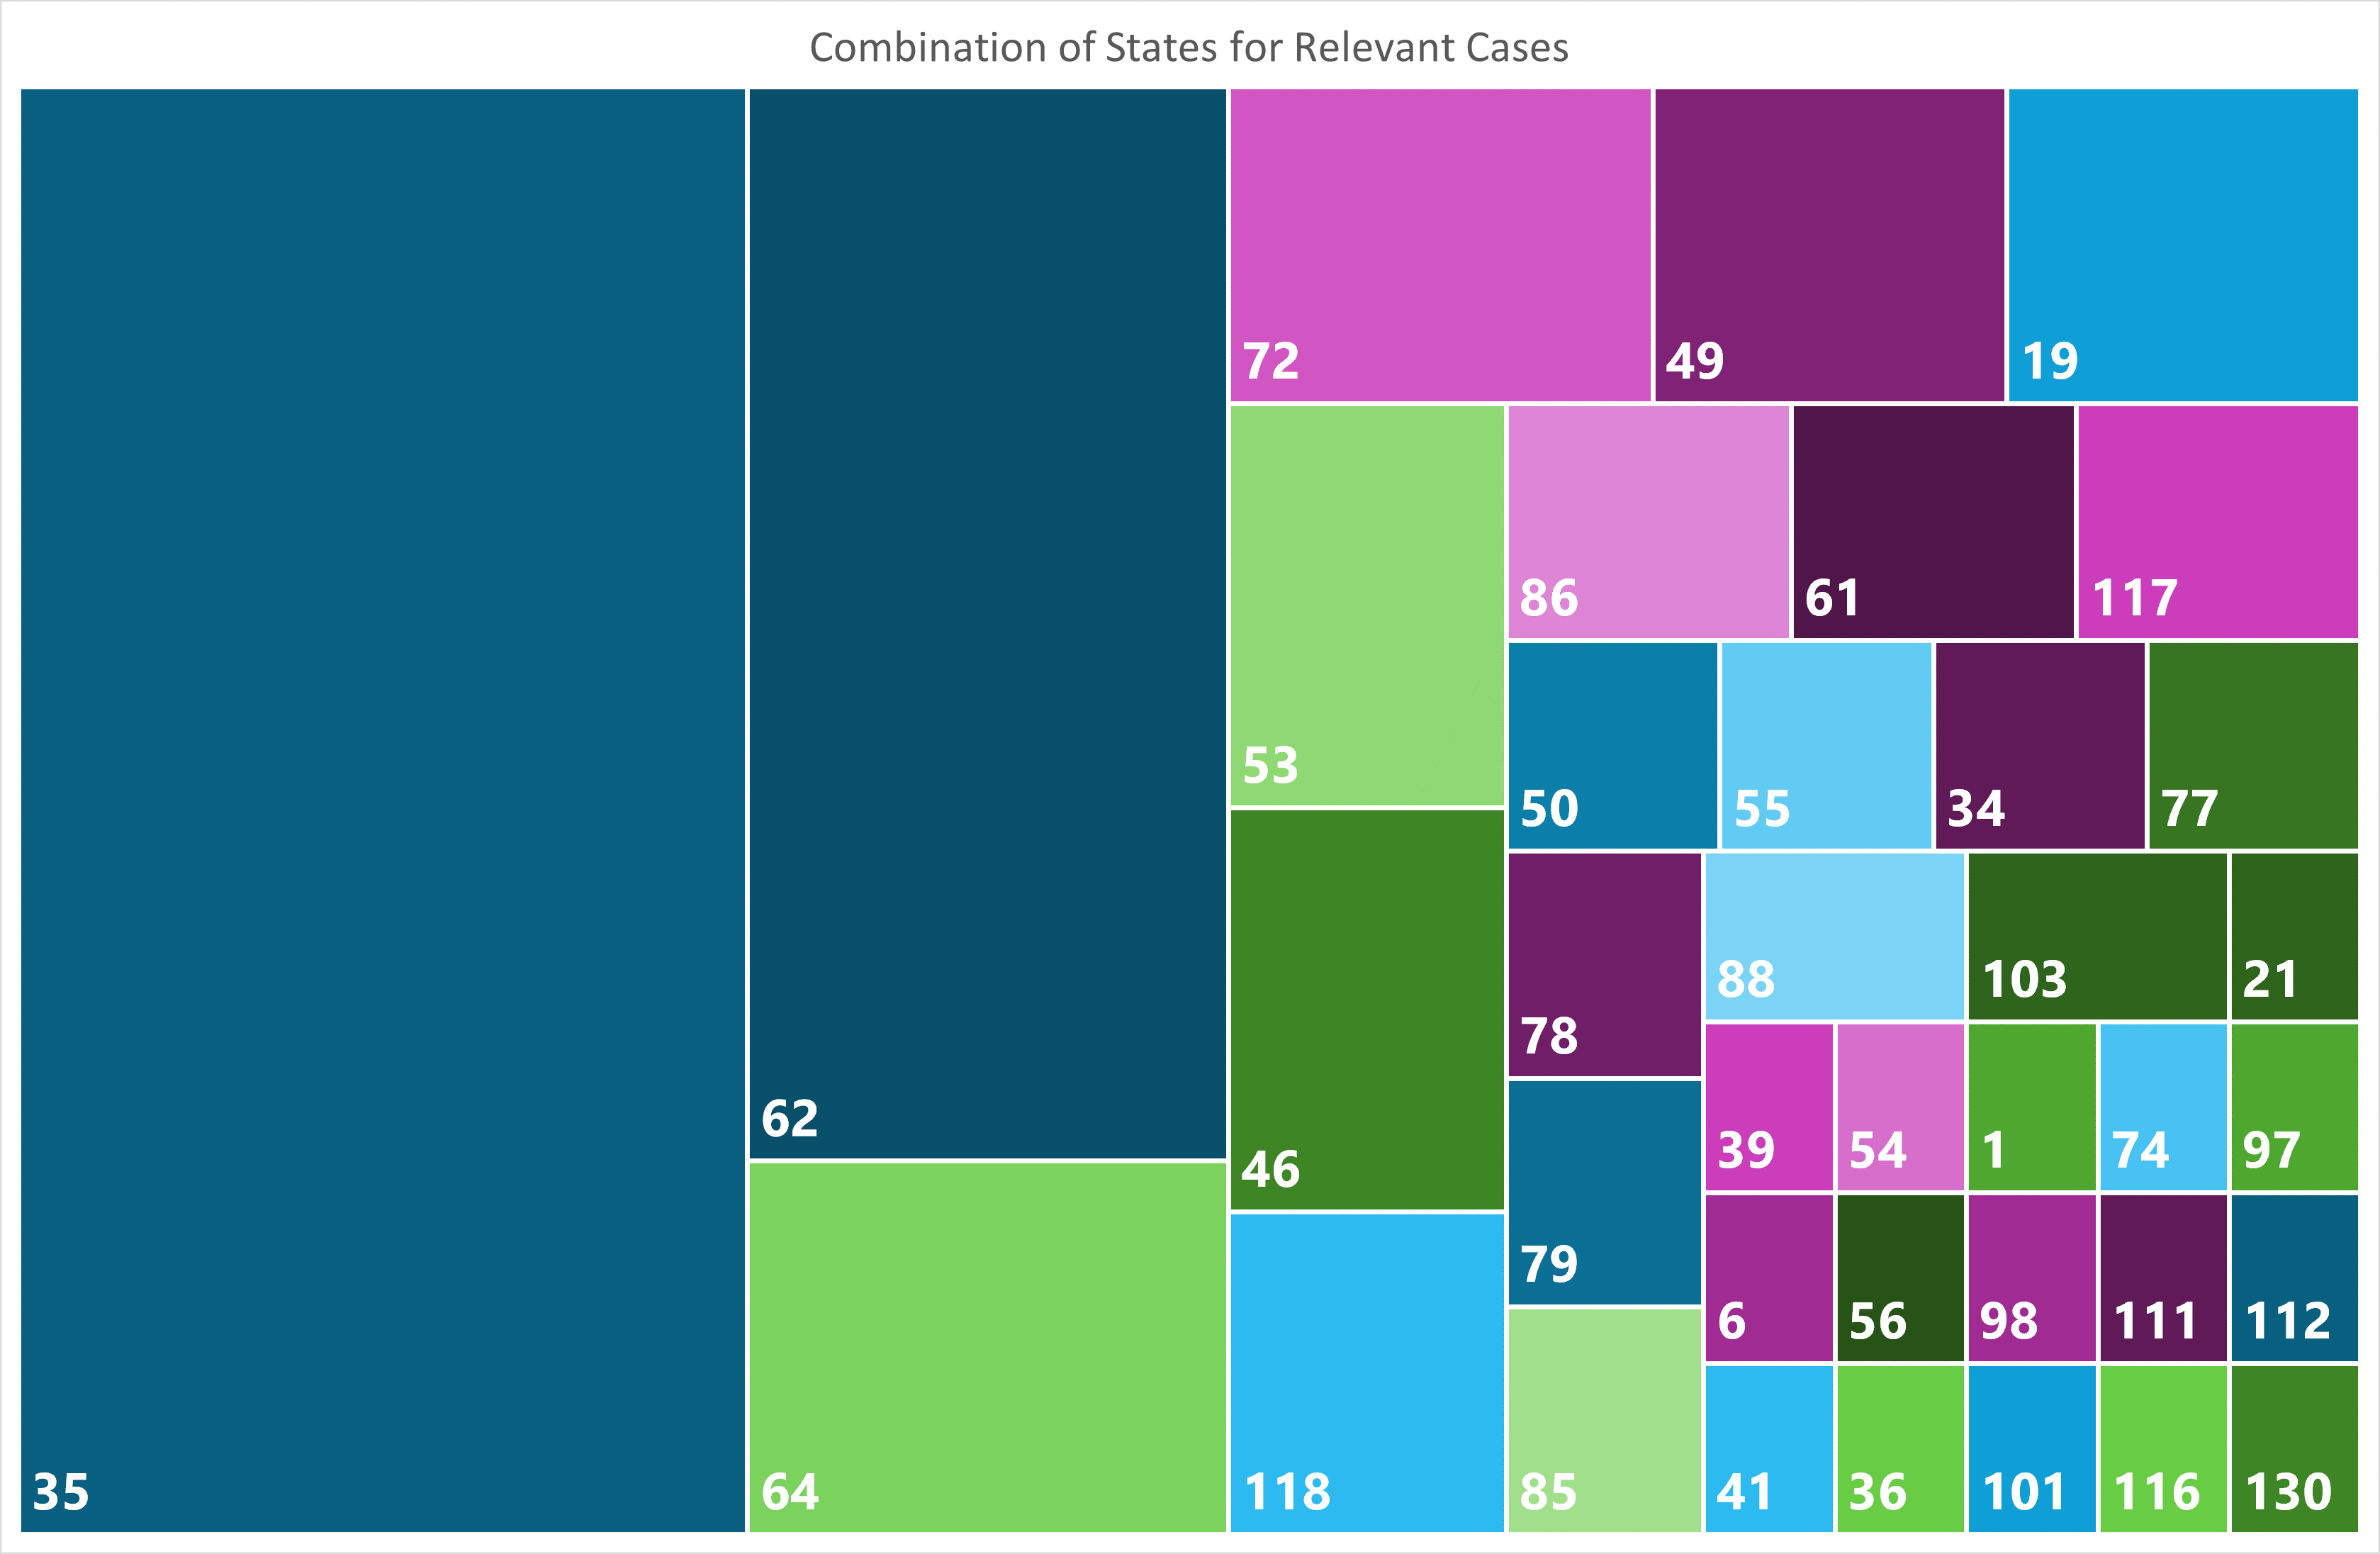
\includegraphics[width = 1\textwidth]{Abbildungen/Combination_of_States.png}
    \caption{Distribution of Combination of states for relevant cases}
\end{figure}

\begin{table}[H]
\begin{tabular}{lcc} 
\multicolumn{1}{c}{Incursion   on} & Combination of   states & Number of   incursions \\ 
Intersecting   runway              & 49                      & 5                      \\ 
Intersecting   runway              & 53                      & 5                      \\ 
Intersecting   runway              & 50                      & 2                      \\ 
Intersecting   runway              & 77                      & 2                      \\ 
Intersecting   runway              & 78                      & 2                      \\ 
Intersecting   runway              & 79                      & 2                      \\ 
Intersecting   runway              & 103                     & 2                      \\ 
Intersecting   runway              & 54                      & 1                      \\ 
Intersecting   runway              & 55                      & 1                      \\ 
Intersecting   runway              & 56                      & 1                      \\ 
Intersecting   runway              & 74                      & 1                      \\ 
Intersecting   runway              & 101                     & 1                      \\ 
Intersecting   runway              & 130                     & 1                      \\ 
Intersecting   runway              & Total                   & 26                     \\ 
Single runway                      & 35                      & 16                     \\ 
Single runway                      & 62                      & 3                      \\ 
Single runway                      & 64                      & 1                      \\ 
Single runway                      & 72                      & 1                      \\ 
Single runway                      & 46                      & 3                      \\ 
Single runway                      & 19                      & 1                      \\ 
Single runway                      & 117                     & 2                      \\ 
Single runway                      & 34                      & 2                      \\ 
Single runway                      & 85                      & 1                      \\ 
Single runway                      & 88                      & 1                      \\ 
Single runway                      & 39                      & 1                      \\ 
Single runway                      & 116                     & 1                      \\ 
                                   & Total                   & 33                     \\ 
\end{tabular}
\caption{Combination of states on intersecting runways}
\end{table}

Taking a closer look at the incursions that occurred on intersecting runways shown on table ---, it can be observed that out of the 59 incursions, 26 correspond to runway incursions that took place on intersecting runways, while 33 of them did not involve the intersecting runway. The incursions involving the intersecting runway appear to be significant, as they account for almost half of the incursions on these runways. This is consistent with what would be expected, as an intersecting runway adds to the complexity of the layout. It introduces combinations of OSED states that correspond to incursions that are not possible on single or parallel runways.  

\subsection{A and B Runway incursions involving a commercial aircraft and a ground vehicle}

\begin{figure}[H]
    \centering
    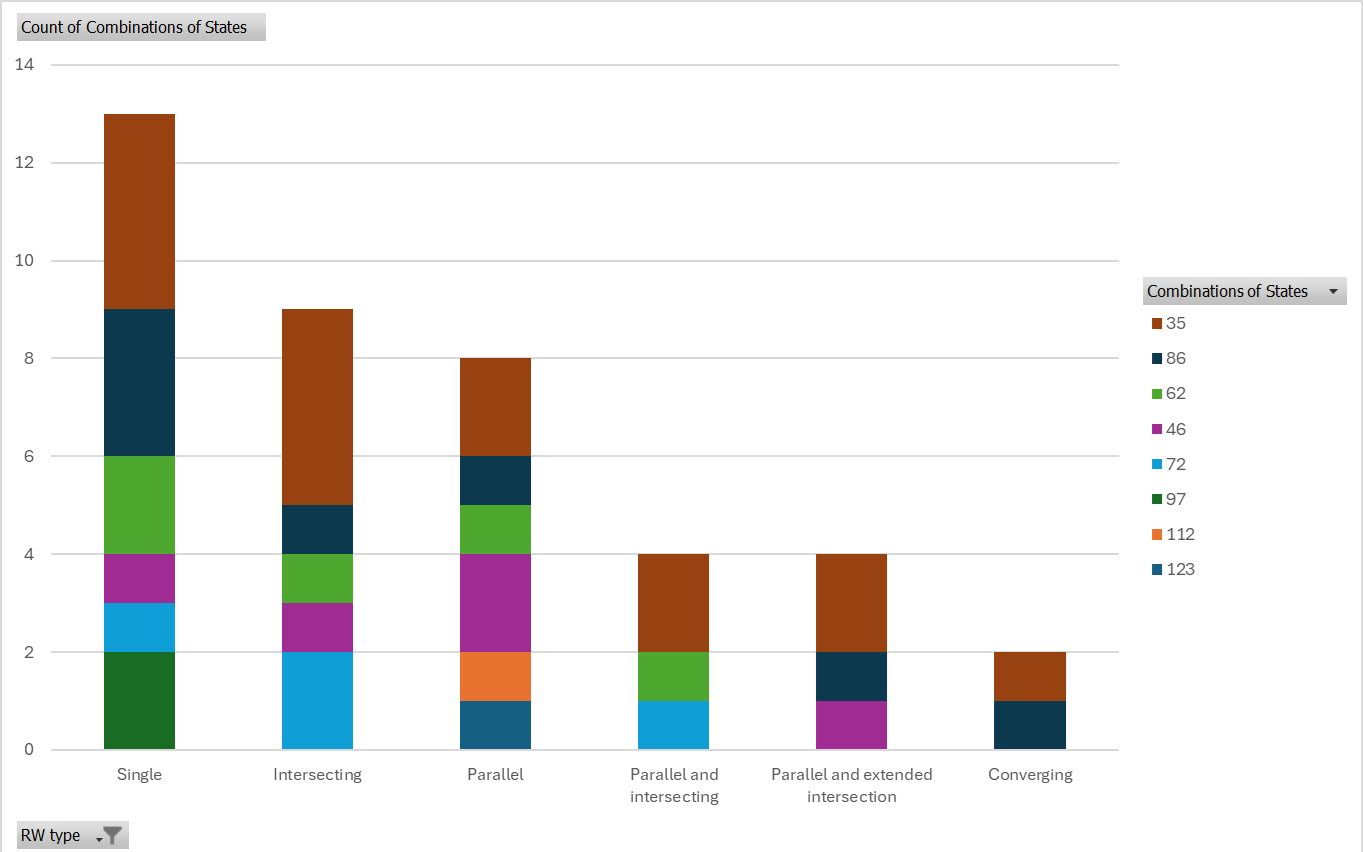
\includegraphics[width = 0.8\textwidth]{Kapitel/Commercial x ground vehicle - incursions by geometry.png}
    \caption{Count of incidents of A and B Severity involving a commercial aircraft and a ground vehicle}
    \label{fig:enter-label}
\end{figure}

Figure --- shows the combination of states by runway geometry of the 40 incursions involving a commercial aircraft and a ground vehicle. Contrary to the incidents involving two aircrafts, the most common runway geometry in this case is single runways, followed by intersecting and parallel runways. This is to be expected as even though intersecting runways add complexity, it is unlikely that a vehicle will be taxiing in a runway, they mostly just cross them unless they are doing surveillance or maintenance activities. All of the 40 incidents are a single runway incursions. 
\chapter{Conclusion}
\label{ch:grundlagen}

Wichtige Info: Als Compiler muss \textbf{LuaLaTeX} verwendet werden. Auch in ShareLatex!

\section{Discussion}
\section{Recommendations}
\section{Conclusion}

%%%%%%%%%%%%%%%%%%%%%%%%%%%%%%%%%%%%%%%%%%%%%%%%%%%%%%%%%%%%%%%%%%%%%%%%%
% Literatur %%%%%%%%%%%%%%%%%%%%%%%%%%%%%%%%%%%%%%%%%%%%%%%%%%%%%%%%%%%%%
%%%%%%%%%%%%%%%%%%%%%%%%%%%%%%%%%%%%%%%%%%%%%%%%%%%%%%%%%%%%%%%%%%%%%%%%%
%\phantomsection

%\addcontentsline{toc}{chapter}{\bibname} %Literaturverzeichnis zum Inhaltesverzeichnis hinzufügen
%\raggedright
% \sloppy %Damit die URLS nicht über den Rand hinausstehen

\printbibliography 


%%%%%%%%%%%%%%%%%%%%%%%%%%%%%%%%%%%%%%%%%%%%%%%%%%%%%%%%%%%%%%%%%%%%%%%%%
% Abbildungs- unf Tabellenverzeichnis %%%%%%%%%%%%%%%%%%%%%%%%%%%%%%%%%%%
%%%%%%%%%%%%%%%%%%%%%%%%%%%%%%%%%%%%%%%%%%%%%%%%%%%%%%%%%%%%%%%%%%%%%%%%%
\listoffigures
\listoftables



%%%%%%%%%%%%%%%%%%%%%%%%%%%%%%%%%%%%%%%%%%%%%%%%%%%%%%%%%%%%%%%%%%%%%%%%%
% Anhang %%%%%%%%%%%%%%%%%%%%%%%%%%%%%%%%%%%%%%%%%%%%%%%%%%%%%%%%%%%%%%%%
%%%%%%%%%%%%%%%%%%%%%%%%%%%%%%%%%%%%%%%%%%%%%%%%%%%%%%%%%%%%%%%%%%%%%%%%%
\appendix

\addcontentsline{toc}{chapter}{Anhang}
\renewcommand{\thesection}{\Alph{section}}
\counterwithin{figure}{section}
\addtocontents{toc}{\protect\setcounter{tocdepth}{1}} 	%-1: nur Kapitel "Anhang" wird im Inhaltsverzeichnis gezeigt. 
														%1: Sections werden angezeigt



\chapter*{Attachments}\label{chapter_anhang}

\section{Anhang Eins}
Hier ist der Anhang

\subsection{Anhang Eins.Eins}

\section{Anhang Zwei}




\end{document}
